\chapter{La régulation de l’expression}
{\hypersetup{linkcolor=GREYDARK}\minitoc}
\label{chap:regulation-de-expression}

Chez les organismes multicellulaires, l’activité des gènes est contrôlée à plusieurs niveaux et par de nombreux systèmes de régulation \citep{maston_transcriptional_2006}. Cette régulation peut se faire avant la transcription, par exemple par des modifications épigénétiques qui contrôlent l’accessibilité de la séquence, ou après la transcription, par exemple par la régulation de la stabilité des \acrshort{ARN} messagers. Une partie essentielle du contrôle de l’expression des gènes s’effectue cependant au niveau transcriptionnel, sur lequel je me suis concentré pendant ma thèse.

\section{Organisation de l’ADN dans le noyau}
\label{sec:organisation-ADN}

Dans les cellules eucaryotes, l’information génétique est organisée en une structure complexe, la chromatine, constituée d'\acrshort{ADN} et de nombreuses protéines \citep{kornberg_chromatin_1992}. Il s’agit d’une structure qui assure un degré de compaction dynamique de l’ADN et entraîne une accessibilité variable de la séquence aux machineries protéiques régulant les fonctions essentielles des génomes comme la réplication, la recombinaison, la réparation ou la transcription \citep{felsenfeld_controlling_2003}. La compaction de la chromatine peut être observée à de nombreuses échelles (Figure \ref{fig:Fig4}), mais je m’intéresserai ici plus particulièrement à son unité la plus fondamentale : le nucléosome. Il s’agit du premier niveau de compaction de la chromatine, qui contient 146 ou 147 nucléotides enroulés autour d’un complexe de quatre histones différentes, chaque histone étant présente en double exemplaire pour former un octamère d’histones. Les histones forment une famille de protéines spécialisées dans la formation des nucléosomes et sont parmi les protéines les plus conservées chez les eucaryotes \citep{sandman_diversity_1998}. Leurs extrémités sont la cible de modifications post-traductionnelles (méthylation, acétylation, phosphorylation...) qui peuvent affecter la structure de l’histone. De telles modifications peuvent influencer l’accessibilité de la séquence d’ADN y étant enroulée, ainsi que les interactions protéines-protéines de la chromatine. L’organisation de l’ADN dans le noyau par sa compaction et les modifications de la chromatine forment ainsi un des premiers mécanismes impliqués dans la régulation de la transcription des gènes.

\begin{figure}[h]
 \centering
 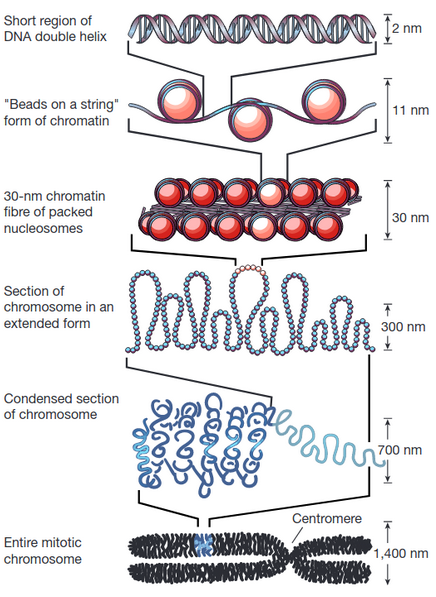
\includegraphics[width=0.5\textwidth, page=1] {figures/introduction/fig4.png}
 \caption[Organisation de l'\acrshort{ADN} au sein de la structure chromatinienne.]{
 \textbf{Organisation de l'\acrshort{ADN} au sein de la structure chromatinienne.}
 De haut en bas. Une région en double hélice d'\acrshort{ADN}. Le premier niveau de compaction est le nucléosome, dans lequel l'\acrshort{ADN} est enroulé autour de l'extérieur d'un octamère d'histone. Les nucléosomes sont reliés les uns aux autres par de courtes portions d'\acrshort{ADN} de liaison. Au niveau d'organisation suivant, la chaîne de nucléosomes est repliée et condensée en une fibre d'environ 30 nm de diamètre. Ces fibres sont ensuite repliées en structures d'ordre supérieur. Aux niveaux de structure au-delà du nucléosome, les détails du repliement sont encore incertains. Tirée de \citet{felsenfeld_controlling_2003}. \\
 }
 \label{fig:Fig4}
\end{figure} 

\section{La régulation transcriptionnelle}
\label{sec:reg-transcription}

La régulation transcriptionnelle des gènes est présente dans tous les systèmes cellulaires \citep{ptashne_regulation_2005}. Elle se fait grâce à des éléments \gls{trans}-régulateurs, c'est-à-dire des séquences d’ADN dont les produits (protéines ou \acrshort{ARN}s) circulent dans le noyau des cellules et interagissent avec différents loci pour réguler l’expression de leurs gènes cibles. Les produits des éléments \gls{trans}-régulateurs, aussi appelés \textit{trans}-facteurs, peuvent se fixer sur des séquences \gls{cis}-régulatrices, qui quant à elles vont avoir une action locale sur le même chromosome que leurs gènes cibles. La transcription des gènes chez les eucaryotes est ainsi un processus complexe qui nécessite l’orchestration d’interactions entre de multiples protéines, des \acrshort{ARN}s et des séquences d’ADN \citep{maston_transcriptional_2006,ong_enhancer_2011}.

\subsection{Les facteurs \textit{trans}-régulateurs}
\label{subsec:elem-trans}

\subsubsection{Les facteurs de transcription}
\label{subsubsec:facteur-trans}

Les facteurs de transcription (\acrshort{FT}s) sont des protéines qui se fixent généralement à l’ADN grâce à leur affinité avec de courtes séquences spécifiques de 6 à 16 nucléotides appelées des motifs de fixation, pouvant être plus ou moins nombreux et/ou stricts. Ces protéines contrôlent l’initiation, la progression ou l’arrêt de la transcription d’un ou plusieurs gènes. Chaque \acrshort{FT}, selon son ou ses motifs de fixation, peut se fixer à de nombreuses séquences dans le génome et ainsi participer à la régulation de plusieurs gènes à la fois. Les régions où se fixent les \acrshort{FT}s sont généralement enrichies en plusieurs sites de fixation de \acrshort{FT}s différents et sont appelées des séquences \gls{cis}-régulatrices.\\

Les \acrshort{FT}s forment généralement des complexes avec d’autres \acrshort{ARN}s ou protéines (ARN polymérase, enzymes, \acrshort{FT}s,…). Leurs modes d’actions sont variés, ils peuvent par exemple participer aux recrutements de différentes molécules impactant la régulation des gènes cibles ou participer à l’élaboration de boucles de chromatine. Le rôle fonctionnel d’un \acrshort{FT} est très dépendant de la diversité et de la concentration de plusieurs autres co-facteurs dans les cellules. Un même \acrshort{FT}, en présence de différents co-facteurs, pourra agir différemment ou sur l’expression de différents gènes ce qui le rend potentiellement très \gls{pleiotrope}. C’est alors la combinaison de plusieurs facteurs de transcription fixés sur une même séquence qui a un effet particulier sur les gènes cibles dans chaque type cellulaire. \\

On estime actuellement qu’il existe plus de 1500 gènes codants pour des facteurs de transcription dans le génome humain \citep{wingender_tfclass_2018}. Selon leurs motifs de fixation, les \acrshort{FT}s peuvent réguler un nombre très variable de gènes. De plus, la transcription de ceux-ci étant elle-même régulée, le patron d’expression des \acrshort{FT}s peut être variable, ceux-ci peuvent être spécifiques à un type cellulaire jusqu'à largement ubiquitaire.

\subsubsection{Les ARNs non-codants}
\label{subsubsec:ARN-noncodant}

La régulation de l’expression des gènes par des éléments agissant en \gls{trans} se fait également par le moyen d’\acrshort{ARN}s non-codants. En effet, la transcription d’un très grand nombre de gènes dans les génomes eucaryotes résulte en \acrshort{ARN}s ne codant pas pour des protéines. Certains de ces \acrshort{ARN}s participent à la régulation de l’expression des gènes. Les micro-\acrshort{ARN}s, composés d’une vingtaine de bases, sont les \acrshort{ARN}s non-codants dont les modes d’action sont peut-être les mieux compris \citep{bartel_micrornas_2004}. Ceux-ci se fixent de manière complémentaire aux \acrshort{ARN}s messagers produits par leurs gènes cibles. Après fixation, les microARN peuvent initier un clivage de l’\acrshort{ARNm} en plusieurs morceaux, ce qui déstabilise sa structure et entraîne une dégradation rapide. Cette fixation peut également perturber ou empêcher la traduction des \acrshort{ARNm} en protéine, inhibant alors l’expression des gènes cibles \citep{bartel_micrornas_2004}. De la même façon que les \acrshort{FT}s, les micro-\acrshort{ARN}s peuvent influencer l’expression d’un nombre très variable de gènes, pour certains jusqu’à plusieurs centaines de gènes. Bien que seulement un faible nombre soit caractérisé et validé expérimentalement, il existerait plus de 2000 micro-\acrshort{ARN}s dans le génome humain \citep{alles_estimate_2019}.\\

Les longs \acrshort{ARN}s non-codants, qui peuvent être composés de plusieurs milliers de bases, sont également une classe importante de régulateurs de l’expression des gènes. Ils peuvent agir à la manière des facteurs de transcription, en participant à la formation de complexes moléculaires ou en recrutant d’autres co-facteurs au niveau de l'initiation et l’élongation de la transcription. Par exemple il a été proposé que l’ARN non codant HOTAIR, participe à la modification de la chromatine dans la région des gènes \textit{HoxD} et interagit avec un complexe Polycomb répressif pour inhiber l’expression des gènes \citep{rinn_functional_2007}.

\subsection{Les séquences \textit{cis}-régulatrices}
\label{subsec:elem-cis}

Les séquences \gls{cis}-régulatrices sont des régions non-codantes de l’ADN qui régulent la transcription d’un ou plusieurs gènes selon leur accessibilité, leurs marques épigénétiques et les facteurs de transcription qui y sont fixés. Elles sont essentielles pour contrôler où, quand et comment un gène cible est activement transcrit. On distingue les promoteurs des gènes, situés immédiatement en amont du gène qu’ils régulent, et les éléments \gls{cis}-régulateurs plus distaux (Figure \ref{fig:Fig5}).

\begin{figure}[h]
 \centering
 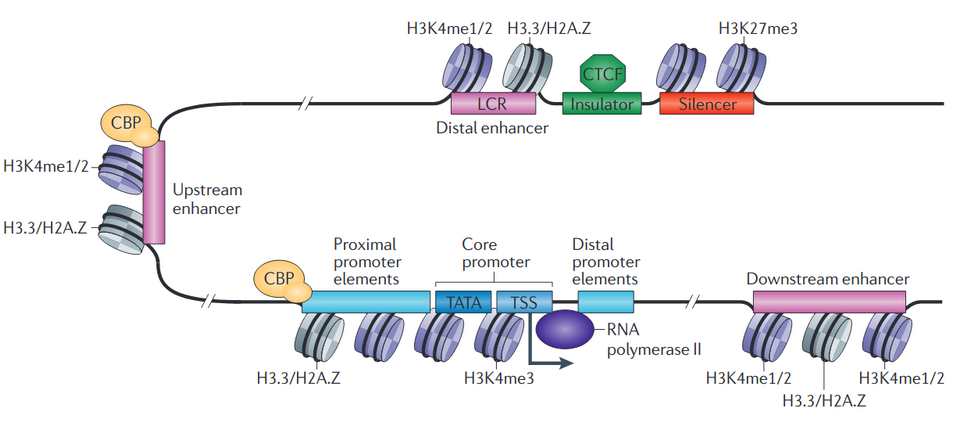
\includegraphics[width=0.8\textwidth, page=1] {figures/introduction/fig5.png}
 \caption[Diversité des éléments \gls{cis}-régulateurs.]{
 \textbf{Diversité des éléments \gls{cis}-régulateurs.}
 La séquence promotrice d'un gène (rectangles bleus) est généralement découpée en trois régions de tailles variables: proximale, centrale et distale, et contiennent notamment des sites de fixation de facteurs de transcription. La région centrale contient la séquence TATA qui permet la fixation de l'\acrshort{ARN} polymérase II et le site d'initiation de la transcription du gène (\acrshort{TSS}). La transcription d'un gène peut également être régulée par de nombreuses séquences en amont ou en aval, dont des \glspl{amplificateur} (rose), des \glspl{inhibiteur} (rouge) ou des isolateurs (vert). La présence de modifications sur les histones des nucléosomes (palets bleu et gris) et la présence de certaines protéines (jaune) au niveau de la chromatine permettent de détecter les séquences \gls{cis}-regulatrices et de mesurer leur activité. 
 
 Abréviations : CBP = Cyclic AMP-responsive element-Binding Protein. H3K4me1/2 = histone H3 mono- or dimethylation at lysine 4; H3K4me3 = histone H3 trimethylation at lysine 4; H3K27me3 = histone H3 trimethylation at lysine 27; H3.3/H2A.Z = histone variants H3.3 and H2A. Tirée de \citet{ong_enhancer_2011}.
 }
 \label{fig:Fig5}
\end{figure} 

\subsubsection{Les promoteurs des gènes}
\label{subsubsec:prom}

Les séquences principales de la régulation transcriptionnelle sont les promoteurs des gènes. La plupart des promoteurs contiennent une séquence spécifique d’une trentaine de nucléotides connue sous le nom de boîte TATA permettant la liaison de l’ARN polymérase II, essentielle à la transcription du gène. La présence au niveau du promoteur de certains facteurs de transcription dits “basaux” comme IIB est également nécessaire pour placer et stabiliser la polymérase avant d’initier la transcription \citep{kostrewa_rna_2009}. Ces facteurs se fixent spécifiquement sur des régions du promoteur d’environ 1 kb qui peuvent être caractérisées par leur enrichissement en dinucléotides \acrshort{CpG}, appelés îlots \acrshort{CpG} \citep{down_computational_2002, deaton_cpg_2011}. La méthylation des cytosines sur ces dinucléotides peut jouer un rôle important dans la compaction de l’ADN et alors influencer l’expression des gènes y étant associés \citep{moore_dna_2013}. De plus, l’ARN polymérase II ne se fixe pas sur tous les promoteurs accessibles du génome en même temps. Son recrutement et sa stabilisation sur les promoteurs dépend de l’accessibilité de la séquence mais également d’autres séquences \textit{cis}-régulatrices plus éloignées.

\subsubsection{Les éléments \textit{cis}-régulateurs distaux}
\label{subsubsec:cis-reg}

Les éléments \gls{cis}-régulateurs distaux sont des séquences capables de fixer des combinaisons de facteurs de transcription et pouvant interagir avec les promoteurs de gènes de manière spécifique via des complexes de protéines et/ou des repliements de la chromatine. Selon les facteurs de transcription qui s’y fixent, ces éléments peuvent être de trois types : \glspl{amplificateur} de l’expression des gènes (“enhancer” en anglais), \glspl{inhibiteur} de l’expression réduisant l’activité des gènes, et isolateurs qui permettent d’isoler certaines régions du génome pour limiter l’interaction des gènes avec d’autres séquences (Figure \ref{fig:Fig5}) \citep{maston_transcriptional_2006}. Dans ce manuscrit, je me concentrerai principalement sur les éléments \gls{cis}-régulateurs identifiés comme \glspl{amplificateur}, qui représentent la catégorie la mieux connue à ce jour. Cependant, il est nécessaire de garder à l’esprit que les éléments \gls{cis}-régulateurs sont très modulables. Une même séquence agissant comme \gls{amplificateur} dans un tissu pourra agir comme \gls{inhibiteur} dans un autre avec une combinaison différentes de facteurs de transcription y étant fixés \citep{gisselbrecht_transcriptional_2020, huang_enhancer-silencer_2022}. De plus les relations fonctionnelles entre un gène et un élément \gls{cis}-régulateur peuvent fortement dépendre des \glspl{condition} biologiques de la cellule. \\

La localisation génomique des éléments \gls{cis}-régulateurs est très hétérogène. Ils peuvent être situés à proximité de la séquence des promoteurs, en amont ou en aval \citep{maniatis_regulation_1987}. Mais ils peuvent aussi se situer à plus grande distance jusqu’à plusieurs mégabases des gènes qu’ils régulent \citep{visel_chip-seq_2009}. Ils peuvent également se situer dans les introns des gènes, comme c’est le cas d’un \gls{amplificateur} de \acrshort{SHH} nommé \acrshort{ZRS} situé dans un intron du gène \textit{LMBR1} à plus de 800kb de \acrshort{SHH} (Figure \ref{fig:Fig6}.A) \citep{lettice_long-range_2003}. Les gènes les plus proches d’un élément \gls{cis}-régulateur ne sont donc pas nécessairement les cibles de celui-ci. Il existe différents mécanismes pour rapprocher spatialement un \gls{amplificateur} de son promoteur cible. Ce rapprochement peut se faire à travers la mise en place de complexes protéiques ou par la formation de boucles de la chromatine, ces deux mécanismes n’étant pas exclusifs (Figure \ref{fig:Fig6}.B).\\

\begin{figure}[h]
 \centering
 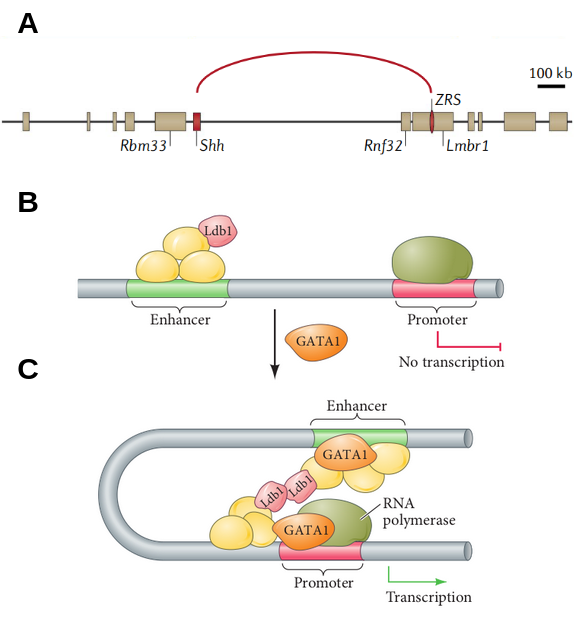
\includegraphics[width=0.7\textwidth, page=1] {figures/introduction/fig6.png}
 \caption[Interaction à grande distance entre promoteur et \gls{amplificateur}.]{
 \textbf{Interaction à grande distance entre promoteur et \gls{amplificateur}.}
 \textbf{A.} Localisation génomique du gène \acrshort{SHH} et de son \gls{amplificateur} \acrshort{ZRS} situé à plus de 800kb dans un intron du gène \textit{LMBR1}.
 \textbf{B et C} Schéma de la formation d'une boucle de chromatine entre un \gls{amplificateur} (vert) fixant des facteurs de transcription et le promoteur d'un gène (rouge) fixant l'\acrshort{ARN} polymérase II. Dans cet exemple c'est le facteur de transcription GATA1 qui assure la liaison entre les deux séquences pour permettre la transcription du gène.\\
 }
 \label{fig:Fig6}
\end{figure}

Les \glspl{amplificateur} sont souvent essentiels au recrutement de la machinerie d’initiation de la transcription mais aussi au déplacement de l’ARN polymérase du promoteur vers le corps du gène, permettant l’élongation de la transcription \citep{zippo_histone_2009}. Ils contrôlent l’efficacité et le taux de transcription d’un gène cible à partir de son promoteur. La transcription chez les eucaryotes fonctionne de manière discontinue, avec des cycles d’activité entrecoupés par des périodes d’arrêts \citep{chubb_transcriptional_2006, raj_stochastic_2006}. L’activité d’un \gls{amplificateur} et/ou l’action conjointe de plusieurs éléments peuvent augmenter la fréquence des ces cycles d’activité. De plus, la transcription des gènes eucaryotes nécessite la décompaction de la chromatine afin d’augmenter l’accessibilité de l’ADN à d’autres protéines comme la polymérase et les facteurs de transcription. Cette tâche peut également être initiée par les \glspl{amplificateur} en fixant des facteurs de transcription. Ces derniers peuvent recruter à leur tour des enzymes de modification des histones ou encore des complexes de remodelage de la chromatine pour altérer sa structure. Il a aussi été montré que les \glspl{amplificateur} peuvent être transcrits en des \acrshort{ARN}s non-codants ou \acrshort{eRNA} (pour “enhancer-RNA” en anglais) \citep{santa_large_2010}. La concentration des \acrshort{eRNA} est corrélée positivement avec l’activité de l’\gls{amplificateur}, mais aussi avec la production d’\acrshort{ARNm} des gènes cibles. Ceci suggère que les \acrshort{eRNA} sont produits lorsqu’ils sont en contact avec le promoteur d’un gène activement transcrit \citep{cheng_genome-wide_2015}. Cette production de transcrits \acrshort{eRNA} pourrait être un simple effet collatéral de la présence de l’ARN polymérase II sur la séquence de l’\gls{amplificateur}. L’\gls{amplificateur} serait alors transcrit mais le produit de cette transcription n’aurait pas de fonction en lui-même \citep{struhl_transcriptional_2007}. Plusieurs études suggèrent cependant que certains de ces \acrshort{eRNA} pourraient jouer des rôles importants dans la régulation de la transcription des gènes situés en \gls{cis}, c'est à dire sur le même chromosome, notamment par leur capacité à recruter des protéines de modification de la chromatine \citep{wang_reprogramming_2011, arnold_diversity_2020}. Une certaine classe de \acrshort{eRNA} a également montré une capacité d’induire et de stabiliser des contacts spécifiques entre promoteurs des gènes et éléments \gls{cis}-régulateurs sans l’intermédiaire de protéine de remodelage de la chromatine \citep{wang_reprogramming_2011}. Finalement, certains \acrshort{eRNA} plus stables et donc moins vite dégradés, pourraient agir comme régulateurs de gènes localisés sur un autre chromosome (en \gls{trans}) en se fixant de manière spécifique sur d’autres \glspl{amplificateur} \citep{cajigas_evf2_2018}. Les mécanismes de fonctionnement des \glspl{amplificateur} ne sont pas encore parfaitement connus mais sembleraient donc être très variés. Ceux-ci peuvent en effet agir comme attracteurs de facteurs de transcription, régulateurs de la machinerie de transcription, modificateurs de la chromatine, inducteurs de boucle d’ADN et régulateurs en \gls{trans}.

\subsection{Contribution des mécanismes en \textit{trans} et en \textit{cis}}
\label{subsec:contrib-cis-trans}

L’importance relative de la régulation en \textit{trans} et en \gls{cis} dans l’expression des gènes peut-être complexe à évaluer. Dans une expérience originale de transgénèse, Wilson et collaborateurs ont testé si les différences d’expression des gènes entre la souris et l’humain étaient dirigées par la séquence génétique ou par l’environnement nucléaire \citep{wilson_species-specific_2008}. Suite au transfert du chromosome 21 humain dans les cellules d’une souris transgénique, ils ont observé que la distribution des sites de fixation des facteurs de transcription sur ce chromosome dans les cellules de souris était similaire à la distribution observée dans les cellules humaines. De même, le patron d’expression des gènes localisés sur le chromosome 21 était similaire à celui observé chez l’humain, et non pas à celui des gènes homologues chez la souris. Cette observation est également valable pour le patron d’épissage des gènes codants pour des protéines \citep{barbosa-morais_evolutionary_2012}. Ainsi, la séquence génétique et donc les éléments \gls{cis}-régulateurs semblent être majoritairement responsables du patron d’expression et d’épissage de ces gènes et non pas les facteurs \gls{trans}. Les différences interspécifiques de l’environnement cellulaire et des éléments agissant en \gls{trans}, tels que les facteurs de transcription ou certains \acrshort{ARN} non-codants, joueraient des rôles secondaires. Ceci semble alors indiquer que, même si les sites de fixation en \gls{cis} ont pu évoluer entre les deux espèces, les facteurs agissant en \gls{trans} présentent une forte conservation évolutive. Ce résultat est attendu car les facteurs de transcription possèdent de nombreuses fonctions distinctes et sont sous une forte sélection purifiante \citep{wray_evolutionary_2007}. Des modifications de leurs séquences engendreraient des conséquences majoritairement délétères sur la valeur sélective de l’organisme. \\

Des changements d’expression de certains régulateurs agissant en \gls{trans} pourraient néanmoins participer aux différences du niveau d’expression des gènes. C’est par exemple le cas pour des microARNs dont la différence d’expression expliquerait une part importante de la divergence d’expression de leurs gènes cibles dans le cerveau des primates \citep{hu_microrna_2011}. L’émergence spécifique d’éléments agissant en \gls{trans} pourrait également permettre des changements de l’expression de gènes et potentiellement avoir un rôle important dans l'évolution phénotypique. Par exemple, le microARN miR-934 spécifique des primates et exprimé lors de la neurogénèse chez l’humain est associé à des changements majeurs du patron d’expression de plusieurs gènes impliqués dans la prolifération et la différentiation des neurones \citep{prodromidou_microrna-934_2020}.

\section{Identification et caractérisation des séquences \textit{cis}-régulatrices}
\label{sec:identif-cis}

Au cours de ma thèse, je me suis concentré sur les séquences \gls{cis}-régulatrices, qui sembleraient être les plus susceptibles de contribuer aux changements de l’expression des gènes. Un des premiers enjeux est alors de détecter ces séquences non-codantes dans les génomes. De nombreuses méthodes existent actuellement pour détecter, identifier et caractériser des séquences qui pourraient potentiellement être impliquées dans les changements d’expression des gènes (Figure \ref{fig:Fig7}). Elles permettent de prédire, plus ou moins précisément, des séquences \gls{cis}-régulatrices candidates. Elles ont dévoilé l’existence de plusieurs centaines de milliers d’\glspl{amplificateur} dans les génomes, dépassant largement le nombre de gènes protéiques. Ces découvertes démontrent l’importance de la régulation de la transcription en tant que premier niveau de contrôle du génome et donc des fonctions de l’organisme. Je vais ici détailler quelques-unes des grandes catégories d’approches utilisées pour identifier les séquences \gls{cis}-régulatrices et dont certaines ont fourni des données essentielles à mes travaux durant cette thèse. \\

\begin{figure}[h]
 \centering
 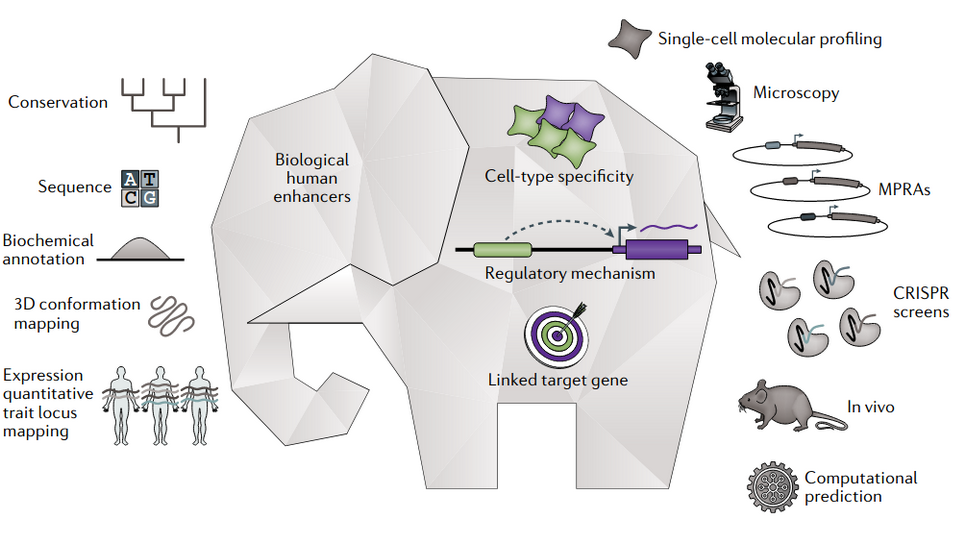
\includegraphics[width=0.9\textwidth, page=1] {figures/introduction/fig7.png}
 \caption[Diversité des méthodes de détection et de caractérisation de la fonction des éléments \gls{cis}-régulateurs.]{
 \textbf{Diversité des méthodes de détection et de caractérisation de la fonction des éléments \gls{cis}-régulateurs.}
 Dans une revue récente, Gasperini et collaborateurs font une analogie entre les différentes méthodes qui tentent de décrire les éléments \gls{cis}-régulateurs et un ancien compte indien où des aveugles tentent de décrire un éléphant en touchant chacun une partie différente. L'ensemble des méthodes, aussi hétérogènes et biaisées soit-elles peuvent être complémentaires et permettent d'obtenir différents aperçus d'une même réalité. Tirée de \citet{gasperini_towards_2020}.
 }
 \label{fig:Fig7}
\end{figure}

\newpage
\subsection{Approches computationnelles}
\label{subsec:approch-comput}

\subsubsection{Association génotype-phénotype}
\label{subsubsec:geno-pheno}

La prédiction d’éléments \gls{cis}-régulateurs peut d'abord s'effectuer par l’association de variations génotypiques à des variations phénotypes. En analysant les séquences génomiques de plusieurs individus conjointement avec une mesure d’un trait phénotypique on peut corréler la fréquence d’une variation génétique avec le trait d'intérêt. Par exemple, la variation d’un nucléotide ou SNP (Single Nucleotide Polymorphism) peut être corrélée à la variation d’un trait quantitatif, on parlera alors de QTL (Quantitative Trait Locus). Lorsque le trait quantitatif auquel on s’intéresse est le niveau d’expression d’un gène, on parlera d’eQTL (expression QTL). Ces méthodes ne cherchent pas spécifiquement des éléments \gls{cis}-régulateurs mais toute séquence ou mutation associée à un trait, les eQTLs peuvent ainsi se situer dans des gènes comme dans des régions non-géniques. Dans ce dernier cas, ils peuvent signaler la présence d'éléments régulateurs. Les mécanismes moléculaires entre un eQTL et les variations de l’expression d’un gène ne peuvent pas être déterminés par cette méthode, ceux-ci pouvant se faire à l’ensemble des niveaux de régulation. \\

C’est notamment par des études d’association entre génotypes et phénotypes qu’au début des années 90 a été découverte la région contenant un \gls{amplificateur} du gène \acrshort{SHH}. Cet \gls{amplificateur} est spécifique du bourgeonnement des membres, et est appelé \acrshort{ZRS} pour “Zone of polarizing activity Regulatory Sequence”. Les études qui ont permis de découvrir \acrshort{ZRS} cherchaient à comprendre les bases génétiques de certaines malformations congénitales. Elles se basent sur l’analyse du génotype d’individus ou de familles présentant des malformations au niveau des membres chez l’humain comme la triphalangie du pouce, la polydactylie (nombre surnuméraire de doigts) ou plus rarement l’acheiropodie (absence de main et de pied) \citep{hing_linkage_1995, zguricas_clinical_1999}. En comparant les variations de plusieurs marqueurs génétiques, ces études ont pu associer ces malformations à la région 7q36 sur le chromosome 7 humain sans pour autant connaître son rôle régulateur. Parallèlement, l’analyse de l’expression de plusieurs gènes dans des embryons de souris mutantes polydactyles a permis d’identifier une expression anormale du gène \acrshort{SHH} comme potentiellement responsable de ce phénotype \citep{sharpe_identification_1999}. \\

Cependant les méthodes d'associations entre génotype et phénotype permettent seulement de détecter une association statistique entre un ou plusieurs loci et un phénotype donné. Elles sont donc grandement dépendantes du nombre d'individus étudiés et des variations de leurs séquences. Aujourd’hui, avec l’avancée des techniques moléculaires, les associations génotype-phénotype sont appliquées à grande échelle, sur un grand nombre d'individus et sur des génomes complets, améliorant grandement leur pouvoir statistique et donc prédictif. C’est le cas des études dites GWAS (Genome Wide Association Study) qui ont permis d’identifier de nombreuses séquences d’ADN polymorphes entre les génomes humains et étant potentiellement responsables de divers changements moléculaires \citep{lappalainen_evolutionary_2010, bryois_cis_2014}.

\subsubsection{Conservation évolutive}
\label{subsubsec:conserv-evol}

Les études de génomique comparative permettent de détecter des séquences non-codantes conservées à plus ou moins large échelle évolutive. Cette forte conservation peut être le signal d’un rôle fonctionnel important associé à des mécanismes de régulation de l’expression des gènes. Chez les vertébrés par exemple, la comparaison de séquences d’espèces divergentes de plus de 300 millions d’années a révélé des séquences hautement conservées dans les régions non-codantes des gènes \citep{duret_strong_1993}. Il a ainsi été proposé que ces séquences pourraient agir comme régulatrices de l’expression des gènes. Une autre analyse se basant sur les alignements de séquence de plusieurs espèces de mammifères sur le génome humain a montré que de nombreuses séquences non codantes appelées Ultra-Conserved-Elements (UCE) sont mieux conservées que des exons codants et certaines peuvent être retrouvées avec une forte similarité de séquence chez les poissons \citep{bejerano_ultraconserved_2004}. \\

De la même manière, pour \acrshort{SHH} et son \glspl{amplificateur} \acrshort{ZRS}, il a été montré que la séquence et la localisation dans le 5ème intron de \textit{LMBR1} de \acrshort{ZRS} sont très conservées entre l’humain, la souris et le poulet, et cette comparaison évolutive a permis de définir plus précisément sa région fonctionnelle à environ 1,2 kb (Figure \ref{fig:Fig8}) \citep{lettice_long-range_2003, sagai_elimination_2005}. De plus, malgré les différences morphologiques importantes entre les membres et les nageoires, un élément \gls{cis}-régulateur homologue de \acrshort{ZRS} est présent chez les poissons. La similarité de séquence entre l’élément  identifié chez le poisson et son homologue chez la souris a permis d’estimer le cœur fonctionnel de l’\gls{amplificateur} à environ 200 pb.

\begin{figure}[h]
 \centering
 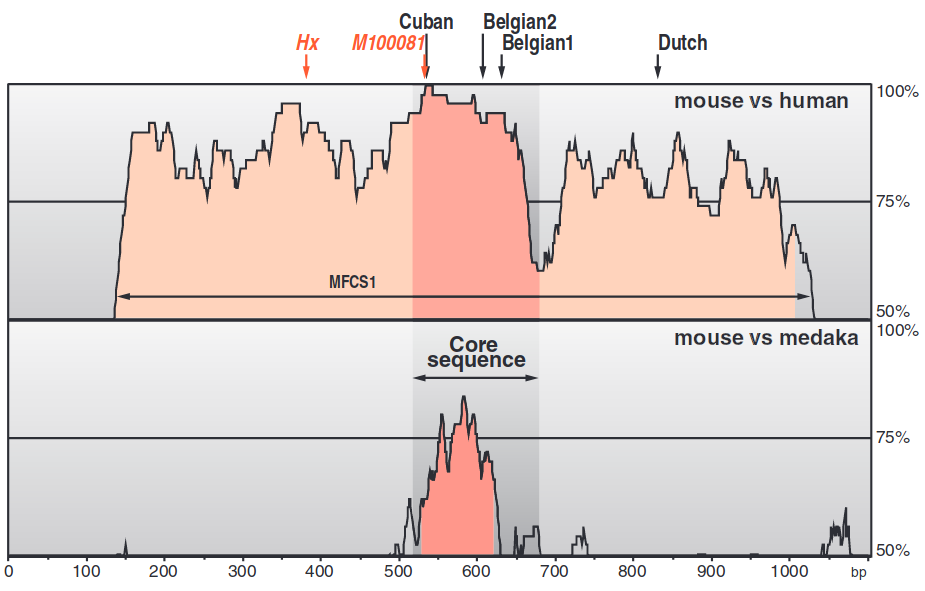
\includegraphics[width=0.8\textwidth, page=1] {figures/introduction/fig8.png}
 \caption[Conservation de la région contenant l'\gls{amplificateur} \acrshort{ZRS} (anciennement MFCS1) de la souris.]{
 \textbf{Conservation de la région contenant l'\gls{amplificateur} \acrshort{ZRS} (anciennement MFCS1) de la souris.}
 Pourcentage de similarité de séquence dans une partie de l'intron 5 de \textit{Lmbr1} entre la souris et l'humain en haut et entre la souris et le medaka (\textit{Oryzias latipes}, un poisson) en bas. Les flèches indiquent les sites où des mutations ponctuelles sont connues pour affecter l'expression de \acrshort{SHH} chez la souris (rouge) et chez l'humain (noir).
 MFCS1 = mammals-fishes-conserved-sequence 1.
 Tirée de \citet{sagai_elimination_2005}\\
 }
 \label{fig:Fig8}
\end{figure}

\subsection{Approches expérimentales}
\label{subsec:approch-expe}

\subsubsection{Ouverture de la chromatine et accessibilité de l’ADN}
\label{subsubsec:ouverture-chroma}

Les premières méthodes pour localiser les éléments fonctionnels actifs ont été développées à partir de l’identification de régions génomiques hypersensibles au clivage par la DNase I, une protéine dégradant l’ADN \citep{keene_dnase_1981, mcghee_200_1981}. Les régions où des modifications locales de la structure de la chromatine perturbent la compaction de l’ADN, comme les promoteurs de gènes activement transcrits, sont plus accessibles et donc plus faciles à digérer par la DNase I. Il a par la suite été montré que les sites hypersensibles à la DNase I (DHSs) sont généralement des régions de moins de 250 nucléotides et sont des marqueurs pour plusieurs catégories d'éléments \gls{cis}-régulateurs, y compris les promoteurs et les \glspl{amplificateur} \citep{felsenfeld_controlling_2003}. Le développement de méthodes de séquençage en haute résolution de ces sites, comme le DNase-seq, a ensuite permis de produire des cartes de l’état de la chromatine à l’échelle du génome entier. Grâce à cette technique par exemple, il a été démontré que dans les cellules T CD4+ humaines, plus de 80\% des DHSs sont localisés en dehors des promoteurs et des exons \citep{boyle_high-resolution_2008}. De plus les DHSs sont enrichis en variants associés à des changements phénotypiques ou à des maladies génétiques, ce qui conforte l’hypothèse d’un rôle majeur dans la régulation des gènes \citep{maurano_systematic_2012}. En combinant des mesures de DNase-seq sur un grand nombre d'échantillons, plusieurs études ont tenté de dresser un répertoire des DHSs du génome humain \citep{thurman_accessible_2012, meuleman_index_2020}. Par exemple, sur plus de 700 échantillons humains, une étude récente a permis de lister plus de 3,5 millions de DHSs et donc de potentiels éléments \gls{cis}-régulateurs \citep{meuleman_index_2020}. Des \textit{consortia} comme ENCODE ou RoadMap Epigenomics, dont l’objectif est d’identifier tous les éléments fonctionnels du génome de l’humain ou de la souris, collectent et mettent à disposition de nombreuses données telles que du DNase-seq avec des protocoles standardisés, ouvrant la voie à de nombreuses études \citep{davis_encyclopedia_2018, roadmap_epigenomics_consortium_integrative_2015}. Nous avons utilisé certaines de ces données comme prédiction des \glspl{amplificateur} au cours de ma thèse dans les travaux que je présenterai dans la Partie \ref{part:chap2} et \ref{part:chap3}. \\

En 2013, une technologie nommée ATAC-seq (“Assay for Transposase Accessible Chromatin with high throughput sequencing”) a été développée pour détecter l’ouverture de la chromatine et donc l’accessibilité de l’ADN de manière plus sensible et à moindre coût \citep{buenrostro_transposition_2013}. Elle se base sur l’activité d’une transposase hyperactive, une enzyme qui va insérer une séquence cible dans toutes les régions du génome où la chromatine est ouverte. Cette séquence intégrée va alors jouer le rôle d'adaptateur pour permettre d’amplifier les régions avoisinantes puis les séquencer à haut débit. Cette technique a facilité l’analyse et la découverte d’éléments \gls{cis}-régulateurs en simplifiant les expérimentations et en les rendant faisable sur un faible nombre de cellules \citep{daugherty_chromatin_2017}. Nous avons utilisé cette technique pour détecter les régions \gls{cis}-régulatrices candidates dans le tubercule génital du poulet et du canard que je détaillerai dans la Partie \ref{part:chap4}. 

\subsubsection{Modification d’histones}
\label{subsubsec:histone}

Les modifications post-traductionnelles des histones peuvent apporter des informations sur les fonctions des séquences. Le développement de méthodes expérimentales utilisant l’immuno-précipitation de la chromatine (ChIP) combinée initialement à des puces à ADN (ChIP-chip) ou plus récemment à du séquençage à haut débit (\acrshort{ChIP-seq}), a permis de déterminer les sites de l’ADN en liaison avec une protéine donnée \citep{ren_genome-wide_2000, barski_high-resolution_2007}. Cette protéine peut être une histone avec des modifications biochimiques précises, un facteur de transcription ou toute autre protéine capable de se fixer à l’ADN \citep{visel_chip-seq_2009}. Avec cette technique, la chromatine est précipitée en utilisant un anticorps spécifique de la protéine d’intérêt, les régions ainsi liées sont récupérées puis séquencées. Grâce à ces données, il a par exemple été montré que des niveaux élevés d'acétylation sur la 27ème lysine (K27) de l’histone H3 (notée H3K27ac) ou de méthylation sur la 4ème lysine du même histone (H3K4me) sont généralement détectés dans les régions promotrices des gènes actifs (Figure \ref{fig:Fig9})  \citep{bernstein_genomic_2005}. De même, des niveaux élevés de méthylation sur la 27ème lysine de l’histone H3 (H3K27me) sont corrélés à la répression des gènes \citep{lee_control_2006}. Ces modifications peuvent également être détectées dans les régions intergéniques. Les signaux d'acétylation de H3 (H3K27ac par exemple) et la mono-méthylation de H3K4 (H3K4me1) à l'extérieur des régions promotrices ont été corrélés avec la présence d’\glspl{amplificateur} \citep{heintzman_distinct_2007}. De nombreux \glspl{amplificateur}, actifs ou non, ont ainsi pu être prédits par ces marques épigénétiques \citep{creyghton_histone_2010}. Ces dernières ne sont pour autant pas toujours discriminantes de la fonction et de l’activité des séquences qui leur sont associées. Par exemple, des marques très similaires peuvent être présentes sur les promoteurs et les \glspl{amplificateur} actifs comme H3K27ac (Figure \ref{fig:Fig9}). Néanmoins, leur cartographie dans différents types cellulaires permettent de mieux identifier et caractériser les régions fonctionnelles. Les \textit{consortia} ENCODE et RoadMap Epigenomics cités plus haut mettent également à disposition de grands répertoires d’éléments non-codants potentiellement fonctionnels identifiés par ces modifications d’histones \citep{davis_encyclopedia_2018, roadmap_epigenomics_consortium_integrative_2015}.

\begin{figure}[h]
 \centering
 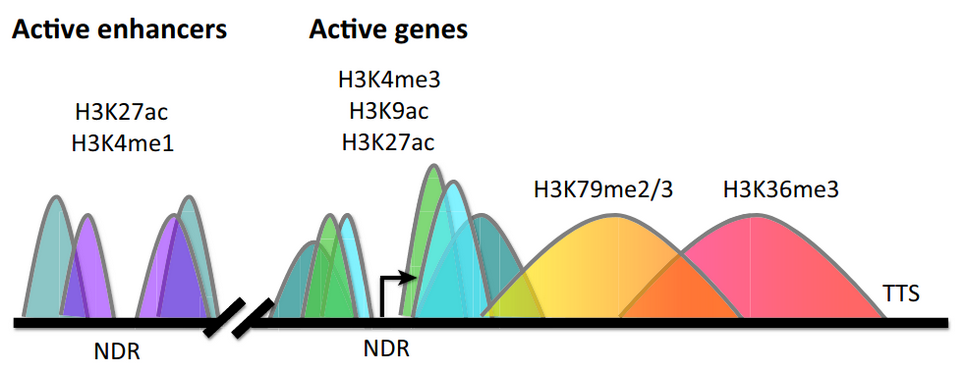
\includegraphics[width=0.8\textwidth, page=1] {figures/introduction/fig9.png}
 \caption[Localisation génomique des modifications d'histone H3 associées à la transcription active des gènes.]{
 \textbf{Localisation génomique des modifications d'histone H3 associées à la transcription active des gènes.}
 Schéma de l'occupation des modifications des histones H3 obtenus par les méthodes d'immunoprécipitation de la chromatine et de séquençage (\acrshort{ChIP-seq}). Les régions en couleur représentent un signal ChIP classique pour des \glspl{amplificateur} ou des gènes actifs.
 Gris, acétylation sur la lysine 27 de H3 (H3K27ac) ; violet, monométhylation sur la lysine 4 de H3 (H3K4me1) ; bleu clair, acétylation sur la lysine 9 de H3 (H3K9ac) ; vert, triméthylation sur la lysine 4 de H3 (H3K4me3) ; jaune, di- et triméthylation sur la lysine 79 de H3 (H3K79me2/3) ; rose/rouge, triméthylation sur la lysine 36 de H3 (H3K36me3). H3K4me3 et H3K9ac sont associés aux régions promotrices des gènes actifs, alors que H3K36me3 et H3K79me3 sont localisés dans les corps des gènes en cours de transcription. H3K27ac se localise à la fois au niveau des promoteurs des gènes actifs et des amplificateurs, et H3K4me1 est principalement enrichi au niveau des amplificateurs.
 Les gènes réprimés présentent des marques de méthylation différentes et pas d'acétylation d'histone (non montré). La flèche indique le site d'initiation de la transcription (\acrshort{TSS}). 
 Abréviations : NDR, région appauvrie en nucléosomes ; TTS, site de terminaison de la transcription. Tirée de \citet{bernstein_genomic_2005}.\\
 }
 \label{fig:Fig9}
\end{figure}

\subsubsection{Transcription des amplificateurs}
\label{subsubsec:eRNA}

Par défaut la présence de l'ARN polymérase II sur une séquence génère des transcrits courts dans les deux orientations (ou brins) de l'\acrshort{ADN} \citep{kim_widespread_2010, andersson_atlas_2014}. Au niveau des promoteurs classiques, des signaux supplémentaires permettent d'assurer l'élongation de la transcription des gènes dans une seule direction. L’ARN polymérase II peut cependant rester pendant un temps plus ou moins long sur les régions promotrices ainsi que sur les \gls{amplificateur} actifs avant l’élongation \citep{rougvie_rna_1988, mayer_pause_2017}. Durant ce laps de temps, ces derniers sont transcrits de manière bidirectionnelle, ce qui permet d'une part de les discriminer des autres transcrits \acrshort{ARN}s et d'autre part de quantifier leur activité. Cependant, même si leur stabilité peut être variable, ces transcrits sont généralement rapidement dégradés \citep{almada_promoter_2013}. Les méthodes classiques de \acrshort{RNA-seq} ne peuvent pas les détecter, mais ils peuvent être capturés et séquencés par des méthodes dédiées. \\

L’une d’elle nommée \acrshort{CAGE} ("Cap Analysis of Gene Expression"), s’appuie sur la capture et l’isolation de la coiffe présente sur l’extrémité 5’ des transcrits matures \citep{shiraki_cap_2003, andersson_atlas_2014}. Contrairement au séquençage \acrshort{RNA-seq} cette méthode cible et enrichit les premières bases des \acrshort{ARN}s, permettant de détecter les transcrits très courts et proches des sites d’initiation de la transcription (\acrshort{TSS}). Une autre technique, GRO-seq ("Global Run-On sequencing"), permet de mesurer de manière très sensible le taux de transcription des séquences engagées avec l’ARN polymérase II active \citep{core_nascent_2008}. Avec cette technique, les cellules sont mises en présence d’un nucléotide spécifique (le 5-bromouridine 5'-triphosphate) qui s'insère dans les \acrshort{ARN}s en cours de transcription. L'ajout de ce nucléotide aux transcrits permet ensuite de les isoler puis de les séquencer à haut débit. Le GRO-seq présente l’avantage de quantifier les fragments de transcrits naissants indépendamment de leur stabilité dans le noyau. Cette technique a notamment permis de détecter plusieurs \glspl{amplificateur} engagés avec un promoteur transcrit \citep{melgar_discovery_2011}. Les techniques de séquençage des éléments \gls{cis}-régulateurs transcrits ont permis d’identifier des \glspl{amplificateur} spécifiques de tissus et/ou de plusieurs stades de développement chez différentes espèces de mammifères, \textit{in vivo} ou \textit{in vitro}. Nous avons également utilisé des données publiques de GRO-seq et \acrshort{CAGE} dans le travail décrit dans la Partie \ref{part:chap3}).

\subsection{Validation fonctionnelle}
\label{subsec:validation}

Bien que de nombreuses méthodes permettent aujourd’hui d’identifier de potentiels éléments \gls{cis}-régulateurs à l’échelle de génomes entiers, il reste important de valider leur fonction exérimentalement et de déterminer précisement leurs impacts sur l’expression des gènes cibles. \\

Avec les contraintes évolutives apparentes des éléments non-codants ultra conservés (UCE) et leur relative proximité aux gènes, les premières études prédisaient déjà l’importance de ces séquences et leurs potentiels rôles dans la régulation de l’expression des gènes. Certains de ces UCE (n=167) ont été testés par des expériences de transgénèse chez des souris \citep{pennacchio_vivo_2006}. Pour tester la fonction de chaque UCE, celui-ci est injecté dans un embryon sous forme de plasmide et est associé avec un gène dit “rapporteur de l’expression” car la présence de ses protéines peut être visualisée par coloration ou fluorescence. Dans cette étude, c’est le gène \textit{LacZ} qui a été utilisé car il possède un promoteur minimal mais nécessite un \gls{amplificateur} actif pour produire des protéines dont l’activité enzymatique colore les cellules en bleu \citep{li_overview_2018}. Cette coloration permet de déterminer si un UCE donné joue effectivement un rôle d’\gls{amplificateur} et si oui dans quels tissus. Cette étude a ainsi montré que 45\% des séquences conservées testées sont des \glspl{amplificateur} de l’expression des gènes qui agissent dans un ou plusieurs tissus dans des embryons de souris au stade 11.5 (Figure \ref{fig:Fig10}) \citep{pennacchio_vivo_2006}. \\


\begin{figure}[h]
 \centering
 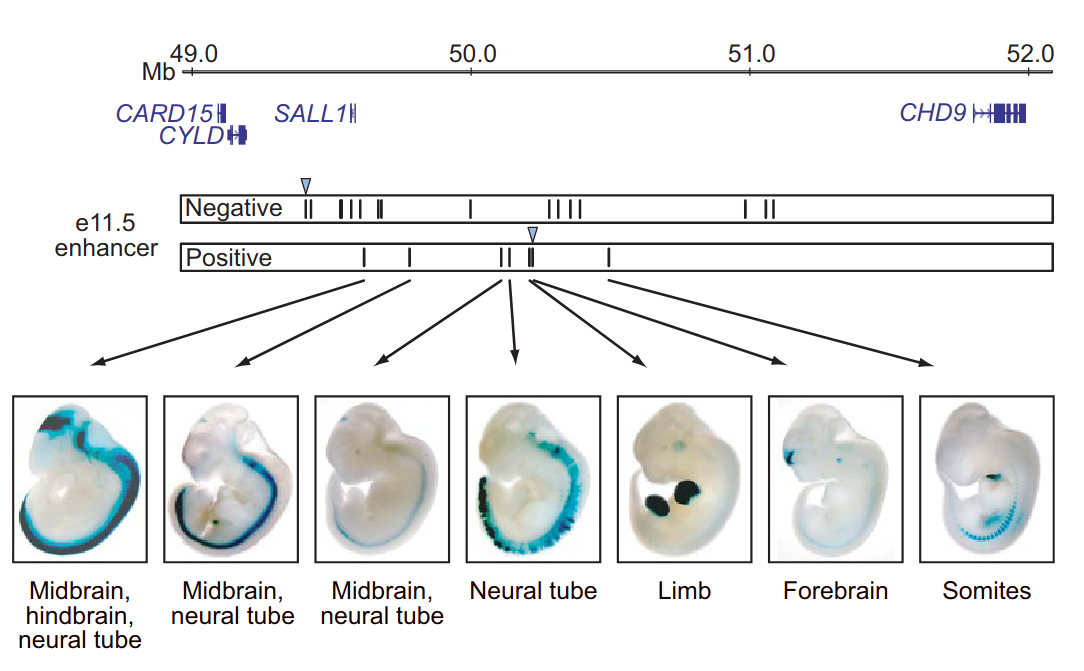
\includegraphics[width=0.8\textwidth, page=1] {figures/introduction/fig10.png}
 \caption[Validation de la fonction régulatrice de séquences non-codantes ultra-conservées.]{
 \textbf{Validation de la fonction régulatrice de séquences non-codantes ultra-conservées.} De haut en bas. Coordonnée génomique d'un fragment humain enrichi en éléments conservés chez le poisson-globe. Position des éléments humains testés dans une experience de transgénèse dans des embryons de souris. Les flèches bleues indiquent les éléments définis comme ultra-conservés. Les éléments sont classés comme "positif" ou "négatif" selon leur rôle d'activateurs de l'expression du gène \textit{LacZ} au 11,5ème jour du développement embryonnaire. Photographies des activités amplificatrices positives, la coloration bleue indique la localisation des protéines \textit{lacZ}. Tirée de \citet{pennacchio_vivo_2006}\\
 }
 \label{fig:Fig10}
\end{figure}

Afin de tester le rôle fonctionnel de l’\gls{amplificateur} \acrshort{ZRS} du gène \acrshort{SHH} et son implication dans les malformations des membres, Lettice et collaborateurs ont également effectué des expériences de transgénèse de la région contenant \acrshort{ZRS} dans des embryons de souris \citep{lettice_long-range_2003}. Cette étude a permis de confirmer le rôle activateur de l’expression de \acrshort{ZRS} dans le développement des membres. Ils ont également pu confirmer que de nombreuses mutations observées à des fréquences élevées dans les génomes d’individus présentant des polydactylies se localisent dans cette région. En effectuant des expériences de transgénèse de la séquence de \acrshort{ZRS} contenant certaines de ces mutations, une autre étude du même groupe a pu identifier un gain d’activité anormale dans plusieurs régions des membres (Figure \ref{fig:Fig11}) \citep{lettice_point_2008}. Cette nouvelle activité de \acrshort{ZRS} dans ces cellules active l’expression de \acrshort{SHH} et entraîne plusieurs malformations des membres. Par ailleurs, il a été montré que la délétion complète de l’\gls{amplificateur} \acrshort{ZRS} chez des souris entraîne des phénotypes similaires à l’inactivation complète du gène \acrshort{SHH} dans les membres, avec d’importantes malformations et des membres tronqués (Figure \ref{fig:Fig11}) \citep{sagai_elimination_2005}. 

\begin{figure}[h]
 \centering
 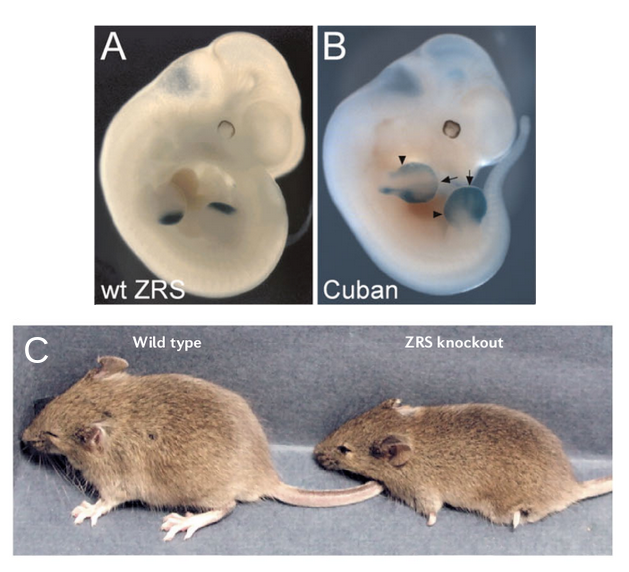
\includegraphics[width=0.6\textwidth, page=1] {figures/introduction/fig11.png}
 \caption[Validation de l'activité de l'\gls{amplificateur} \acrshort{ZRS}.]{
 \textbf{Validation de l'activité de l'\gls{amplificateur} \acrshort{ZRS}.}
 \textbf{A.} Photographie d'une expérience de transgénèse de la séquence normale de \acrshort{ZRS} de la souris dans un embryon de 11,5 jours, l'expression du gène rapporteur \textit{LacZ} (en bleu) a lieu dans la région postérieur des membres. 
 \textbf{B.} Transgenèse de la séquence de \acrshort{ZRS} comportant une mutation identifiée chez des patients atteints de polydactylie (identifiée sur une famille cubaine). Les flèches noires indiquent les régions des membres où une activité anormale est détectée. 
 \textbf{C.} Photographie d'une souris adulte normale et d'une souris aux membres tronqués où la séquence de \acrshort{ZRS} a été retirée du génome.
 Tirées de \citet{lettice_long-range_2003} et de \citep{sagai_elimination_2005}.\\
 }
 \label{fig:Fig11}
\end{figure}

L’importance fonctionnelle de nombreuses séquences \gls{cis}-régulatrices sur la morphologie, la physiologie et le comportement a été démontrée expérimentalement et chez plusieurs espèces \citep{wray_evolutionary_2007}. Cependant, la validation fonctionnelle des éléments \gls{cis}-régulateurs reste complexe et coûteuse. De plus, dans la grande majorité des cas, les relations entre éléments \gls{cis}-régulateurs et gènes sont très spécifiques d’un type cellulaire ou d’un contexte temporel ou environnemental, ce qui rend leur analyse délicate. Ainsi, l’accumulation de prédictions par différentes méthodes ou analyses est nécessaire afin de renforcer la confiance attribuée à chaque élément avant la validation de candidats d’intérêt. La base de données VISTA par exemple propose de recenser les éléments \gls{cis}-régulateurs validés expérimentalement \citep{visel_vista_2007}. Elle permet de confirmer des éléments non-codants prédits par l’accumulation de marques épigénétiques ou par une extrême conservation dans plusieurs espèces de vertébrés. Des expériences d’insertion des séquences prédites avec un marqueur de l’activité dans des embryons de souris sont ensuite menées pour tester leur fonctionnalité. Aujourd’hui plus de 3200 séquences ont été testés \textit{in vivo} chez la souris et plus de 1600 se sont révélés être des \glspl{amplificateur} actifs. \\

D’autres techniques ont également été développées pour tester l'activité amplificatrice d'un grand nombre de séquences en parallèles dans des lignées cellulaires \textit{in vitro}, comme le STARR-seq (“Self-Transcribing Active Regulatory Region sequencing”) ou le MPRA (“Massively Parallel Reporter Assays”) \citep{arnold_quantitative_2014, inoue_decoding_2015}. Celles-ci se basent principalement sur l’insertion d’un gène rapporteur de l’expression combiné à une séquence code-barre unique au niveau de nombreux loci d’intérêt à tester. Les séquences ayant un rôle d’\glspl{amplificateur} de l’expression permettent ainsi au gène intégré d’être transcrit. Après séquençage, il est possible de discriminer les différents transcrits à l’aide des codes-barre et ainsi identifier et quantifier l’activité des éléments \gls{cis}-régulateurs candidats. \\

Finalement, la validation fonctionnelle d’un \gls{amplificateur} n’est pas nécessairement synonyme d’effet direct sur l’expression des gènes. De nombreux mécanismes de compensation peuvent intervenir pour réduire l’effet d’un \gls{amplificateur} ou celui-ci peut ne simplement pas être associé à un gène dans un contexte cellulaire donné.

\section{Les contacts promoteur-amplificateur}
\label{sec:contact}

Pour obtenir un tableau complet du paysage \gls{cis}-régulateur d'un génome, il ne suffit pas d'identifier les éléments \gls{cis}-régulateurs mais il est également nécessaire de définir quels sont leurs gènes cibles. Certains éléments \gls{cis}-régulateurs peuvent se trouver séparés par plus d'un million de nucléotides des gènes qu’ils contrôlent, comme nous l’avons vu pour \acrshort{SHH} et l’\gls{amplificateur} \acrshort{ZRS}. Environ la moitié des éléments \gls{cis}-régulateurs se situeraient à plus de 250 000 paires de base de leur gène cible chez l’humain \citep{montavon_regulatory_2011}. Des repliements particuliers de l’ADN pourraient alors aider à mettre les éléments \gls{cis}-régulateurs en contact avec les promoteurs des gènes cibles pour assurer leurs fonctions régulatrices. De telles boucles de la chromatine ont été observées et permettent de rapprocher physiquement les gènes et les éléments \gls{cis}-régulateurs distaux \citep{tolhuis_looping_2002}. Ces structures, dont les déterminants et les conséquences sont un vaste champ d'étude actuel en biologie moléculaire, pourraient alors être essentielles pour assurer la régulation de l’expression des gènes.

\subsection{Impact sur la transcription}
\label{subsec:impact-transcription}

Différentes équipes ont cherché à comprendre si le contact entre \gls{amplificateur} et promoteur est essentiel à l’initiation de la transcription \citep{carter_long-range_2002}. Elles ont rapporté que les contacts s'établissent en même temps que la transcription des gènes, sans pouvoir distinguer s’ils sont la cause ou la conséquence de l'activation des gènes. Plusieurs études ont alors été menées pour induire expérimentalement un contact physique entre un \gls{amplificateur} et un gène tout en mesurant l’expression de celui-ci. Dans une première expérience, Deng et collaborateurs ont utilisé deux protéines à doigts de zinc (ZFP pour “zinc-finger protein”) se fixant spécifiquement à la séquence promotrice du gène de la Beta-globuline (\textit{Hbb}) de la souris pour l’une et à sa région régulatrice (LCR) pour l’autre \citep{deng_controlling_2012}. Chacune des ZFP est fusionnée avec un co-facteur de transcription LDB1 impliqué dans la formation de boucle d’ADN à grande distance en s’associant deux à deux (Figure \ref{fig:Fig12}.A). Ce contact forcé a entraîné une forte augmentation de la production d’\acrshort{ARNm} de \textit{Hbb}, démontrant que le contact entre le gène et l’\gls{amplificateur} peut augmenter la transcription du gène. Plus précisément, en utilisant le même modèle de contact forcé, Bartman et collaborateurs ont montré que l’augmentation de la fréquence du contact entre le promoteur de \textit{Hbb} et LCR entraîne une augmentation de la fréquence des pics d’activité de transcription du gène mais pas de leur durée \citep{bartman_enhancer_2016}. De plus, en ajoutant une ZFP associée avec LDB1 sur le gène de l’Alpha-globuline voisin de \textit{Hbb}, ce dernier est moins fréquemment transcrit. Cette dernière observation semble indiquer qu’il existerait une compétition des gènes pour le contact avec les \glspl{amplificateur}.

\begin{figure}[H]
 \centering
 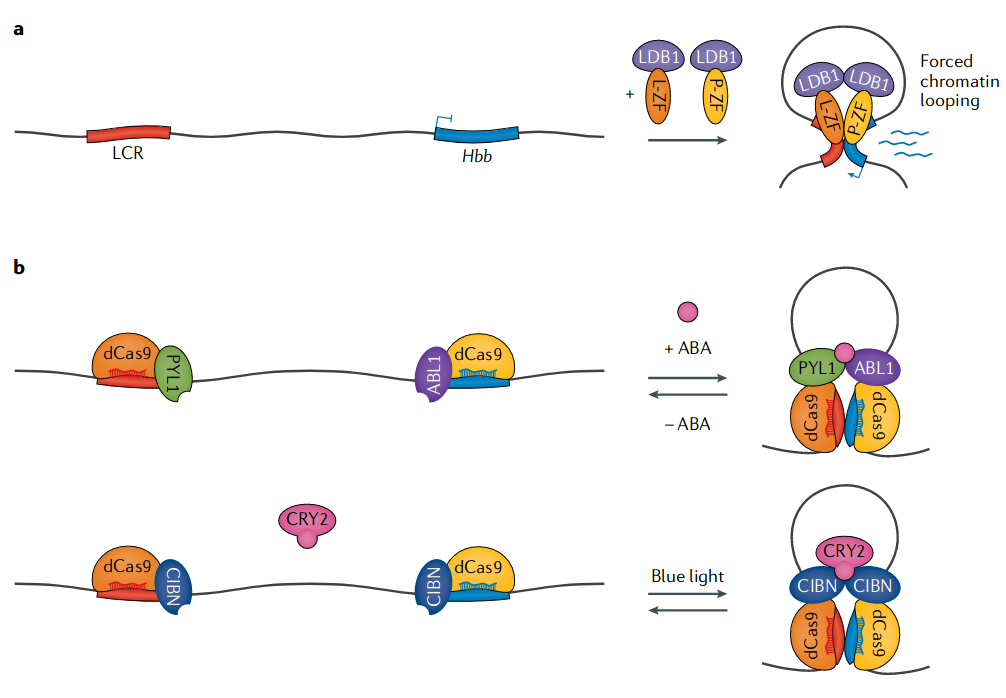
\includegraphics[width=0.8\textwidth, page=1] {figures/introduction/fig12.png}
 \caption[Techniques de contacts forcés entre promoteur et \gls{amplificateur}.]{
 \textbf{Techniques de contacts forcés entre promoteur et \gls{amplificateur}.}
 \textbf{A.} Contact forcé entre le promoteur de la Beta-globuline (\textit{Hbb}) de la souris et son \gls{amplificateur} LCR (locus control region). Des protéines à doigt de zinc fusionnées à une protéine LIM-domain binding 1 (LDB1) ciblent spécifiquement le promoteur de \textit{Hbb} (P-ZF) et la séquence de LCR (L-ZF). Ce contact forcé provoque l'augmentation de la transcription de Hbb \citep{deng_controlling_2012}.
 \textbf{\textbf{B.}} Contacts forcés à partir d'une variation de la machinerie CRISPR éditrice de génome. L'utilisation d'une nucléase-déficiente Cas9 (dCas9) permet de fusionner des protéines au niveau de séquences spécifiques. L'interaction réversible entre ces protéines permet ensuite de rapprocher les régions génomiques auxquelles elles sont fixées. Dans le premier cas, dCas9 est fusionné avec une protéine PYL1 (provenant de \textit{Streptococcus pyogenes}) sur un locus et une protéine ABL1 (provenant de \textit{Staphylococcus aureus}) sur un autre locus. Les deux protéines se dimérisent en présence d'acide abscissique (ABA) ce qui entraine le rapprochement des deux régions génomiques \citep{morgan_manipulation_2017}. Dans le second cas, les dCas9 sont fusionnées à des sous-unités de la protéine CIBN (provenant d'\textit{Arabidopsis thaliana}). En présence de protéines de cryptochrome 2 (CRY2) et de lumière bleu, les protéines CIBN forment un hétérodimère et rapprochent les régions sur lesquelles elles sont fixées \citep{kim_ladl_2019}. Tirée de \citet{schoenfelder_long-range_2019}.\\
 }
 \label{fig:Fig12}
\end{figure}

Pour aller plus loin dans la compréhension de ce mécanisme, des méthodes ont été développées pour forcer un contact entre un gène et son \gls{amplificateur} de manière contrôlable et réversible. Ceci a été possible grâce à l’utilisation d’un dérivé de la célèbre technique d’édition de séquence CRISPR-Cas9, qui fonctionne par l’action de l’enzyme de restriction Cas9 capable de se fixer à une séquence et de la découper en clivant les liaisons entre les nucléotides \citep{doudna_new_2014}. Dans cette approche, deux protéines Cas9 sont artificiellement modifiées pour se fixer à la séquence d’un promoteur pour l’une et d’un \gls{amplificateur} pour l’autre, mais sans les découper. Les Cas9 modifiées (dCas9) sont fusionnés avec des protéines qui, sous l’action d’un intermédiaire extérieur, vont pouvoir se rapprocher ou non (Figure \ref{fig:Fig12}.B). Dans la première étude décrivant cette méthode, l’intermédiaire extérieur est la présence ou non d’acide abscissique (ABA) \citep{morgan_manipulation_2017}. D’autres méthodes ont ensuite été développées, comme l’utilisation de lumière bleue agissant sur le cryptochrome 2 (CRY2) fusionné aux dCas9 et qui permet de rapprocher les loci \citep{kim_ladl_2019}. Dans les deux cas, ce contrôle sur le contact entre les deux séquences a permis de réguler de manière significative la transcription des gènes ciblés. Parallèlement, Bonev et collaborateurs ont découvert non seulement que les contacts entre \glspl{amplificateur} et promoteurs coïncident avec l'activation des gènes au cours de la différenciation des cellules souches de souris, mais aussi qu'ils sont interrompus lorsque les gènes sont réprimés \citep{bonev_multiscale_2017}. La microscopie confocale, couplée à des photographies à intervalle régulier, corrobore ce résultat en permettant de visualiser simultanément la transcription et la proximité entre promoteurs et \glspl{amplificateur} au cours du temps \citep{chen_dynamic_2018}.

\subsection{Formation et maintien des contacts}
\label{subsec:formation-contact}
\subsubsection{Facilitation des contacts : TADs et boucles CTCF}
\label{subsubsec:TAD-boucle}

D’après les contacts de chromatine observés, les génomes des métazoaires semblent être organisés en domaines de quelques mégabases à l’intérieur desquels les interactions entre loci sont facilitées \citep{sexton_role_2015, dixon_topological_2012, rao_3d_2014}. Ces domaines de contact connus sous le nom de \acrshort{TAD} (“Topologically Associating Domains”) permettent de partitionner le génome spatialement \citep{symmons_functional_2014}. Les contacts entre les éléments \gls{cis}-régulateurs et les promoteurs des gènes seraient favorisés à l’intérieur d’un même \acrshort{TAD} alors qu’ils seraient limités entre les \acrshort{TAD}s. Cela permettrait notamment de limiter l’influence d’éléments \gls{cis}-régulateurs non inclus dans un domaine et d’empêcher une activation aberrante des gènes. Ce rôle à la fois facilitateur et isolateur de contact pourrait avoir une importance majeure dans le contrôle de l’expression des gènes. \\

Les frontières de ces domaines sont enrichies en sites de fixation du facteur de transcription CTCF \citep{vietrirudan_comparative_2015}. CTCF est une protéine à doigts de zinc qui se fixe de manière directionnelle à l’ADN grâce à la reconnaissance d’un motif spécifique. Elle a été originellement identifiée comme \gls{inhibiteur} de l’expression de certains gènes \citep{filippova_exceptionally_1996} puis comme \gls{inhibiteur} de l’activité des \glspl{amplificateur} et aujourd’hui comme isolateur de régions d'\acrshort{ADN} \citep{bell_protein_1999}. En agissant conjointement avec la cohésine (un complexe protéique ayant une structure en anneau et de nombreux rôles dans la structuration de la chromatine), les sites de fixation de CTCF permettraient la formation de boucles d’ADN par un principe d’extrusion (Figure \ref{fig:Fig13}) \citep{sanborn_chromatin_2015}. Selon le modèle décrit par Sanborn et collaborateurs, le complexe de cohésine peut se fixer à l’ADN et initier la formation d’une petite boucle. Il est composé de deux sous-unités qui parcourent chacune l’ADN dans des directions opposées, élargissant la boucle de plus en plus. Chaque sous-unité du complexe d’extrusion est composée de protéine CTCF ce qui lui permet de s’arrêter lorsqu’elle rencontre son motif spécifique. Ce dernier n’est pas palindromique et est reconnu seulement dans une direction, de sorte qu’une boucle d’ADN ainsi formée sera composée de CTCF convergents à chacune de ces extrémités. La boucle qui résulte de cette extrusion engendre un domaine dans lequel les régions génomiques peuvent se rencontrer physiquement plus fréquemment. Une protéine nommée WAPL peut ensuite interagir avec la cohésine pour la détacher de l’ADN, ce qui libère le complexe formé et réduit la boucle d’ADN à son état d’origine. Les domaines formés par ce principe d’extrusion pourraient correspondre aux \acrshort{TAD}s observés dans les expériences de contacts de chromatine. \\

\begin{figure}[H]
 \centering
 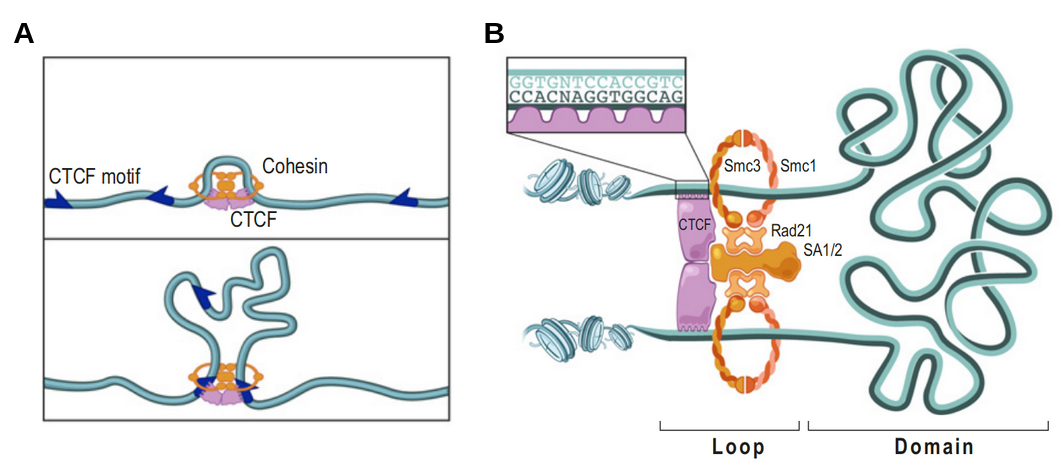
\includegraphics[width=0.8\textwidth, page=1] {figures/introduction/fig13.png}
 \caption[Formation d'une boucle d'\acrshort{ADN} par un principe d'extrusion.]{
 \textbf{Formation d'une boucle d'\acrshort{ADN} par un principe d'extrusion.}
 \textbf{A.} Un complexe protéique composé de deux anneaux de cohésine et de protéine CTCF se place sur l'ADN et initie une boucle. Ce complexe parcourt la séquence et agrandit la boucle jusqu'à la reconnaissance des motifs de CTCF. \textbf{B.} Vue complète de la formation d'un domaine plus large par principe d'extrusion. Tirée de \citet{sanborn_chromatin_2015}.
 \textbf{C.} Schéma de la formation de boucles d'ADN par un principe d'extrusion. \`A mesure que les complexes CTCF parcourent la séquence à divers endroits simultanément, les boucles s'agrandissent.
 \\
 }
 \label{fig:Fig13}
\end{figure}

Plusieurs études expérimentales sont en accord avec un mode de régulation facilitée par les \acrshort{TAD}s. Par exemple, l’intégration de nombreux gènes rapporteurs de l’expression (\textit{LacZ} avec promoteur minimal) dans le génome de la souris a notamment permis de montrer que leurs patrons d’expression sont similaires à ceux des gènes présents dans le même \acrshort{TAD} \citep{symmons_functional_2014}. Cela indiquerait que les éléments \gls{cis}-régulateurs permettent une co-activité des gènes au sein d’un \acrshort{TAD}. De plus, plus de 20\% des \acrshort{TAD}s présenteraient des marques épigénétiques homogènes sur les séquences qui les compose, ce qui assurerait une co-activité des gènes s’y trouvant \citep{le_dily_distinct_2014}. Cependant, dans la majorité des \acrshort{TAD}s des gènes exprimés et réprimés coexistent \citep{le_dily_distinct_2014}. De plus, il a été observé que plus d’un tiers des interactions promoteur-\gls{amplificateur} franchissent les frontières des \acrshort{TAD}s, et que certains contacts cruciaux traversent plusieurs \acrshort{TAD}s \citep{javierre_lineage-specific_2016}. Cette proportion est plus faible qu’attendue par hasard dans un modèle sans \acrshort{TAD}, ce qui confirme en partie leur rôle isolateur, mais suggère que ces domaines ne sont pas des isolateurs absolus \citep{schoenfelder_long-range_2019}. De plus, à l’heure actuelle, les \acrshort{TAD}s sont principalement définis par la fréquence des contacts de chromatine détectés et sont donc avant tout des objets statistiques. Il est par exemple possible de définir des sous-unités de \acrshort{TAD}s imbriquées, ce qui complique d’autant plus leurs délimitations.

\subsubsection{Un modèle complet : sélection-facilitation-spécificité}
\label{subsubsec:modele-complet}

Dans une revue récente, se basant sur les connaissances actuelles sur l’organisation de la structure tridimensionnelle des génomes, Schoenfelder et Fraser proposent un modèle mécanistique complet pour expliquer les processus qui permettent la mise en relation des promoteurs et des \glspl{amplificateur} de manière efficace et sélective \citep{schoenfelder_long-range_2019}. Celui-ci repose sur trois grands axes à différentes échelles (Figure \ref{fig:Fig14}). Dans ce modèle, la première étape permettrait de marquer spécifiquement les régions d’ADN dans chaque type cellulaire à l’aide de modifications épigénétiques (Figure \ref{fig:Fig14}.A). Pour ce faire, des protéines capables de se lier directement à la chromatine condensée seraient dans un premier temps essentielles pour décompacter des régions spécifiques. Le recrutement d’enzymes agissant sur l’état de la chromatine, les modifications d'histones, et la fixation de facteurs de transcription permettraient ensuite de marquer épigénétiquement les gènes et les éléments \gls{cis}-régulateurs pour préparer des sites de liaison pour d’autres protéines. Une seconde grande étape serait la relocalisation dans le noyau de grandes régions génomiques pour faciliter les contacts de la chromatine et la transcription (Figure \ref{fig:Fig14}.B). Notamment de grandes portions chromosomiques seraient déplacées dans des régions du noyau où la transcription est plus importante. De plus, la formation de \acrshort{TAD}s et de plus petites boucles d’ADN permettrait de former des micro-environnements tridimensionnels réduisant l’espace de recherche entre gènes et éléments \gls{cis}-régulateurs. Finalement en dernière étape, la spécificité du contact entre promoteurs et éléments \gls{cis}-régulateurs à l’intérieur d’une boucle d’ADN dépendrait d’éléments \gls{trans}-régulateurs comme les facteurs de transcription ou les \acrshort{ARN}s non-codants (Figure \ref{fig:Fig14}.C). Ceux-ci, fixés sur les séquences, modifieraient plus localement la conformation de la chromatine et rapprocheraient les loci physiquement pour réguler l’expression des gènes.


\begin{figure}[hbt!]
 \centering
 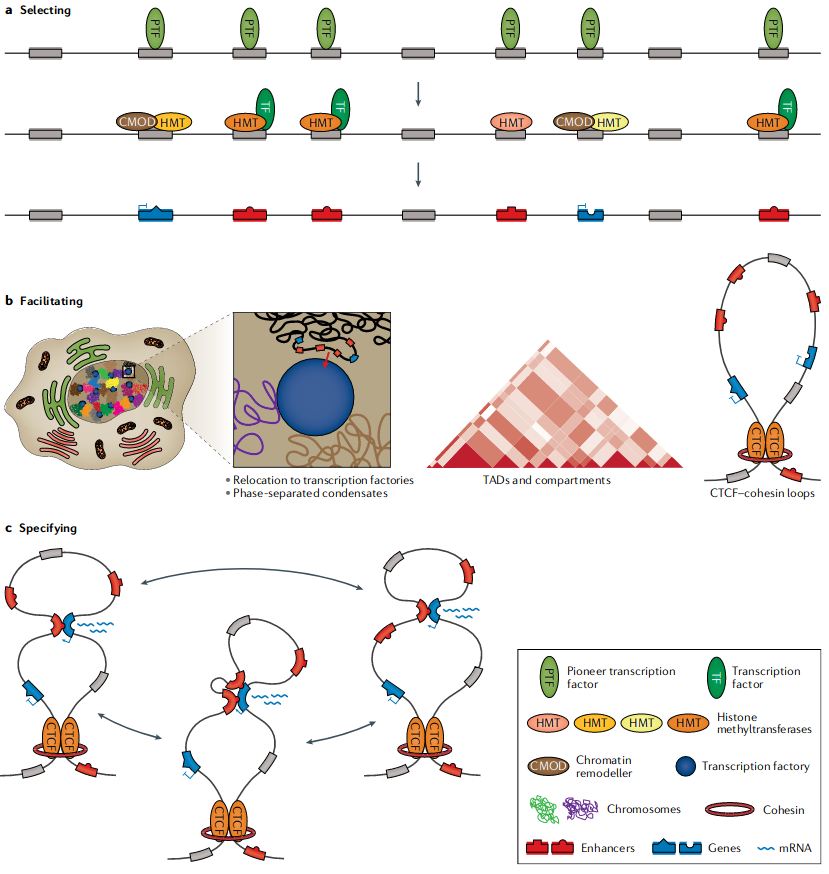
\includegraphics[width=0.8\textwidth, page=1] {figures/introduction/fig14.png}
 \caption[Modèle de sélection, facilitation, spécificité pour les contacts entre promoteur et amplificateur.]{
 \textbf{Modèle de sélection, facilitation, spécificité pour les contacts entre promoteur et amplificateur.}
 \textbf{A.} La \textbf{sélection} : l'action combinée des facteurs de transcription pionniers, des enzymes de remodelage de la chromatine, des facteurs de transcription et des enzymes de modification de la chromatine, telles que les histones méthyltransférases, marque les éléments \textit{cis}-régulateurs spécifiques du type cellulaire par des modifications épigénétiques et la création de sites de liaison pour les protéines de la chromatine. \textbf{B.} La \textbf{facilitation}. La relocalisation de régions génomiques dans des usines de transcription, des domaines d'association topologique (TAD), des compartiments et des boucles créent des micro-environnements qui réduisent l'espace de recherche et augmentent ainsi les chances de rencontre entre les éléments \textit{cis}-régulateurs dans l'espace tridimensionnel. \textbf{C.} La \textbf{spécificité} du contact entre les \glspl{amplificateur} et les promoteurs au sein des domaines ou des boucles est obtenue par des interactions entre facteurs de transcription et éléments \textit{cis}-régulateurs. Ceci permet des transitions dynamiques entre les conformations.
 Tiré de \citet{schoenfelder_long-range_2019}.\\
 }
 \label{fig:Fig14}
\end{figure}


\subsubsection{Contacts spécifiques et préformation}
\label{subsubsec:specifique-preformation}

La mise en place de contacts spécifiques de la chromatine dans les différentes cellules pour permettre leur spécialisation est encore mal comprise. La comparaison de la conformation de la chromatine entre plusieurs types cellulaires d’une même espèce a montré qu’une grande proportion (autour de 40\%) des contacts est spécifique du type cellulaire \citep{javierre_lineage-specific_2016}. Malgré une importante spécialisation, de nombreux contacts sont cependant conservés au cours de la différenciation et sont partagés entre les types cellulaires et plus de 10\% d'entre eux seraient constitutifs  \citep{freire-pritchett_global_2017, rubin_lineage-specific_2017}. Il a également été montré que le regroupement de différentes cellules du sang selon la similarité de leurs contacts reflète les relations de proximité des cellules au cours de la différenciation de la lignée hématopoïétique \citep{javierre_lineage-specific_2016}. Il en va de même pour la spécialisation des cellules de la lignée épidermique \citep{rubin_lineage-specific_2017}. Ces observations suggèrent que les contacts de chromatine changent progressivement au cours de la différenciation cellulaire à partir d'un état précurseur dans les cellules souches. \\

Certains contacts observés dans un type cellulaire donné mettent en relation des éléments \glspl{amplificateur} de l’expression avec des gènes qui ne sont pas actifs dans ce type cellulaire \citep{schoenfelder_pluripotent_2015}. Par exemple, les \glspl{amplificateur} sensibles au facteur de nécrose tumorale dans les fibroblastes humains sont déjà en contact avec les promoteurs des gènes cibles avant la signalisation par ce facteur \citep{jin_high-resolution_2013}. Ces contacts dits pré-formés sont présents avant la transcription des gènes cibles qui s’effectue seulement en réponse à d’autres stimuli. La proximité spatiale entre promoteur et \gls{amplificateur} n’induit donc pas automatiquement une activation du gène, mais pourrait permettre une réponse transcriptionnelle rapide et précise avec l’action combinée d’autres déclencheurs. Les cas de pré-formation de contact de chromatine ne se limitent pas à des voies de signalisation rapides. Le contact entre \acrshort{SHH} et son \gls{amplificateur} \acrshort{ZRS} par exemple a été observé dans de nombreux tissus sans que le gène ne soit exprimé \citep{amano_chromosomal_2009, williamson_shh_2016, ron_promoter-enhancer_2017}. La pré-formation dans ce cas pourrait assurer une proximité constante pour permettre un patron d’expression robuste de \acrshort{SHH} lorsque le gène doit être actif \citep{paliou_preformed_2019}. Plus généralement les contacts pré-formés pourraient maintenir les relations \gls{cis}-régulatrices ayant des impacts majeurs sur le développement ou la survie des individus. 

\subsection{Techniques d’identification des contacts}
\label{subsec:contact-identification}

Identifier la présence de boucles d’ADN et plus généralement la conformation tridimensionnelle de l’ensemble du génome reste encore un défi. De nombreuses avancées et techniques biomoléculaires ont permis d’avoir un aperçu de l’organisation spatiale du génome. Je vais décrire ici quelques-unes de ces techniques et ce qu’elles ont permis de révéler sur l’organisation du génome.

\subsection{Microscopie et cytogénétique moléculaire}
\label{subsec:microscopie}

Les premières observations de l’organisation spatiale du génome ont été rendues possibles par des techniques de microscopie électronique et de cytogénétique moléculaire. Étant très éloigné de ces domaines je ne m'étendrai pas longuement sur celles-ci. Cependant elles ont permis dès le début des années 90 d’observer les premières boucles d’ADN sur des plasmides bactériens entre un facteur de transcription fixé sur la séquence d’un \gls{amplificateur} et l’ARN polymérase II fixée sur le promoteur d’un gène \citep{su_dna-looping_1990}. Une colocalisation spatiale entre \acrshort{SHH} et l’\gls{amplificateur} \acrshort{ZRS} a également pu être observée grâce à un marquage fluorescent par hybridation \textit{in situ} (FISH) au niveau de la séquence de \acrshort{ZRS} et du promoteur de \acrshort{SHH} (Figure \ref{fig:fig15-17}.A-B), \citep{amano_chromosomal_2009}. Plus récemment, des techniques de microscopie avancées comme la microscopie en super-résolution, ont révélé que \acrshort{SHH} et \acrshort{ZRS} sont spatialement proches dans de nombreux tissus mais que la distance entre les deux loci est la plus faible dans la zone d’activité de polarisation durant le développement des membres \citep{williamson_shh_2016}. Finalement, des techniques de microscopie sur cellules vivantes permettent aujourd’hui de visualiser les contacts entre des loci cibles marqués par fluorescence, tout en suivant l’activité de gènes rapporteurs de l’expression en temps réel (Figure \ref{fig:fig15-17}.D). Une étude récente a ainsi montré que la colocalisation entre l’\gls{amplificateur} EVE et le promoteur du gène cible \textit{PP7} corrèle avec l’activité de ce gène dans des cellules de drosophile. La distance entre les deux loci est significativement plus faible lorsque le gène est actif (Figure \ref{fig:fig15-17}.C) \citep{chen_dynamic_2018}. \\

\begin{figure}[h]
 \centering
 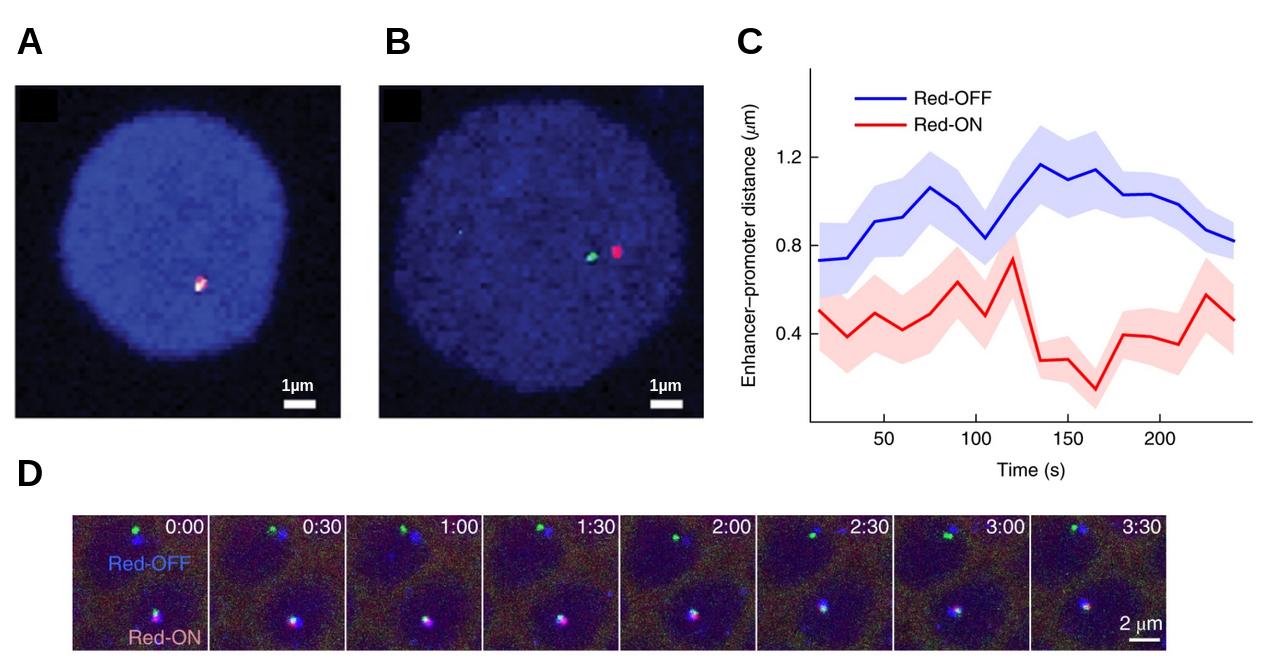
\includegraphics[width=1\textwidth, page=1] {figures/introduction/fig15-17.png}
 \caption[Colocalisation entre gène et \gls{amplificateur} observé par microscopie.]{
 \textbf{Colocalisation entre gène et \gls{amplificateur} observé par microscopie.}
 \textbf{A.} Colocalisation de \acrshort{SHH} et de \acrshort{ZRS} marqués en fluorescence par hybridation \textit{in situ} (FISH) dans des cellules de bourgeons de membres au sein d'un embryon de souris au jour 10.5.
 \textbf{B.} Dans certaines cellules, les deux loci peuvent être séparés.
 \textbf{C.} Suivi temporel de la distance spatiale entre l'\gls{amplificateur} EVE et le promoteur du gène \textit{PP7} dans deux cellules de drosophile lorsque \textit{PP7} est actif (Red-ON) ou inactif (Red-OFF).
 \textbf{D.} 8 photographies suivant 2 noyaux pendant 3min30 où la séquence de EVE (bleue) et le promoteur de \textit{PP7} (vert) sont marqués par FISH. Le noyau en bas présente une activité du gène \textit{PP7} dont les transcrits sont colorés en rouge (Red-ON), alors que dans celui du haut le gène n'est pas actif (Red-OFF).
 Tiréees de \citet{amano_chromosomal_2009} et de \citet{chen_dynamic_2018}.\\
 }
 \label{fig:fig15-17}
\end{figure}

De telles observations ont permis de confirmer un mécanisme de régulation en \gls{cis} par le rapprochement physique des promoteurs et des \glspl{amplificateur} séparés par de grandes régions génomiques. Elles sont essentielles à la compréhension de la dynamique spatiale des génomes.

\subsection{Capture de la conformation de la chromatine}
\label{subsec:HiC}

Ces vingt dernières années, des méthodes expérimentales ont été mises au point pour analyser et prédire plus finement mais aussi de manière plus systématique les contacts de chromatine, et parmi eux les interactions entre gènes et éléments \gls{cis}-régulateurs \citep{dekker_capturing_2002, simonis_nuclear_2006, dostie_chromosome_2006, lieberman-aiden_comprehensive_2009,schoenfelder_pluripotent_2015}. \\

La principale approche expérimentale pour identifier les contacts entre deux loci génomiques est basée sur la liaison par proximité spatiale. Cette approche fait partie des méthodes dites de Capture de Conformation de Chromosome (\acrshort{3C}) (voir \citet{han_3c_2018} pour une revue des méthodes). Elles permettent d’isoler et de séquencer des régions d’ADN se trouvant à proximité spatiale dans le noyau des cellules. En fonction des méthodes de \acrshort{3C} employées, différents contacts entre des loci peuvent être identifiés. On peut les regrouper en quatre grandes classes : un-à-un (analyse du contact entre deux loci ciblés : \acrshort{3C} classique), un-à-tous (analyse de tous les contacts d’un locus cible : \acrshort{3C}-on-Chip, Circular-\acrshort{3C} ou 4C), plusieurs-à-plusieurs (analyse des contacts entre plusieurs loci ciblés : \acrshort{3C}-Carbon-Copy ou 5C) et tous-à-tous (ensemble des contacts à l’échelle du génome : High-throughput-\acrshort{3C} ou \acrshort{Hi-C}) \citep{han_3c_2018}.\\

\begin{figure}[h]
 \centering
 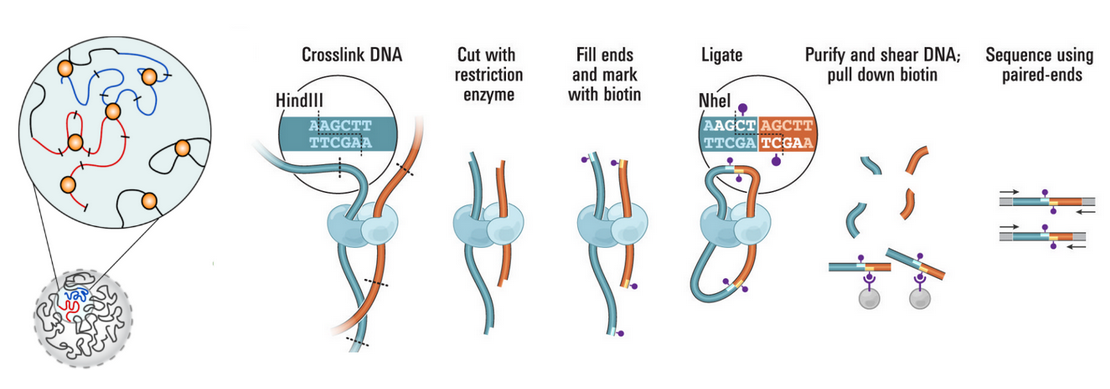
\includegraphics[width=1\textwidth, page=1] {figures/introduction/fig18.png}
 \caption[Principe de capture de la conformation de la chromatine par Hi-C.]{
 \textbf{Principe de capture de la conformation de la chromatine par Hi-C.}
 La conformation de l'ADN dans le noyau des cellules est fixée avec du formaldéhyde, les segments de chromatine proches (représentés en bleu et rouge) sont ainsi liés. Les protéines qui lient les fragments d'ADN sont représentées en bleu clair. La chromatine est ensuite coupée par une enzyme de restriction (HindIII ici) et les extrémités de l'ADN sont marquées par la biotine (ronds violets). Les extrémités sont ensuite liées créant des molécules chimériques. L'ADN est purifié, puis les jonctions biotinylées sont isolées et identifiées par séquençage. Tirée de \citet{lieberman-aiden_comprehensive_2009}.\\
 }
 \label{fig:Fig18}
\end{figure}

Les méthodes de type \acrshort{3C} sont basées sur la fixation au formaldéhyde de la conformation de l’ADN dans le noyau à un instant donné dans le but de figer la chromatine (Figure \ref{fig:Fig18}). Le formaldéhyde entraîne une liaison chimique qui fixe entre eux les loci génomiques qui se trouvent à proximité physique dans le noyau. S'ensuit une étape de digestion de l’ADN par une enzyme de restriction comme HindIII qui reconnaît des sites spécifiques et qui découpe le génome en plusieurs centaines de milliers de fragments de 4 kilobases en moyenne chez l’humain ou la souris. Dans le cas du \acrshort{Hi-C}, chaque extrémité des fragments génomiques est marquée par une biotine. Les fragments découpés sont ensuite ligués de façon circulaire par l’enzyme Nhel, dont les sites de restriction sont en partie communs à ceux de HindIII. Ces fragments circulaires vont alors être purifiés, puis subir des découpes aléatoires par sonication. \`A cette étape, selon la méthode utilisée, différents fragments sont filtrés. Soit sont sélectionnés les fragments contenant les loci ciblés (\acrshort{3C}, 4C, 5C), soit dans le cas du \acrshort{Hi-C}, toutes les séquences contenant des biotines, c’est-à-dire les jointures entre deux fragments de restriction ligués \citep{lieberman-aiden_comprehensive_2009}. Les séquences sélectionnées sont alors amplifiées par PCR puis séquencées à haut débit. La fréquence d'une séquence contenant une partie de deux fragments distincts est ainsi une mesure de la fréquence à laquelle, dans une population cellulaire, les fragments se trouvaient à proximité immédiate au moment de la fixation. \\


La grande limitation du \acrshort{Hi-C} reste la puissance de séquençage. Si l’utilisation de la biotine pour séquencer uniquement les fragments dérivant de contacts de chromatine permet en théorie d’isoler et d’identifier l’ensemble des interactions chromosomiques d’une population de cellules, le nombre de combinaisons possibles est énorme. Les bibliothèques \acrshort{Hi-C}, généralement générées à partir de millions de cellules, sont extrêmement complexes et peuvent représenter près de 100 milliards de séquences indépendantes représentant les jointures de fragments génomiques \citep{belton_hic_2012}. Des méthodes dites de Capture-\acrshort{Hi-C} ont été développées pour traiter et enrichir uniquement un sous-échantillon de ces jointures. Plusieurs techniques d’isolation des interactions existent, certaines combinent les approches C avec une immunoprécipitation de la chromatine pour cibler des fragments contenant des protéines spécifiques, c’est le cas des Chia-Pet ou HiChiP \citep{fullwood_chip-based_2009}. Au cours de ma thèse j’ai utilisé des données produites par une autre approche qui vise à enrichir spécifiquement les jointures obtenus en \acrshort{Hi-C} qui contiennent des promoteurs de gènes, nommée Promoter-Capture-\acrshort{Hi-C} (\acrshort{PCHi-C}) \citep{schoenfelder_pluripotent_2015}. Dans cette approche, des amorces spécifiques sont construites pour s’hybrider par complémentarité avec les extrémités des fragments contenant des promoteurs (près de 40,000 fragments contenant plus de 20,000 promoteurs de gènes pour le génome humain). Ainsi, avant le séquençage, une étape supplémentaire est introduite pour filtrer et amplifier par PCR seulement les jointures faisant intervenir les fragments ciblés. Cette étape de sélection est cruciale car la profondeur de séquençage est limitée, et le signal permettant de détecter une interaction chromosomique peut être entièrement noyé par les interactions les plus fréquentes, abaissant ainsi la sensibilité totale (Figure \ref{fig:Fig19}). Grâce à la technique de \acrshort{PCHi-C}, des catalogues de contacts entre promoteurs des gènes et autres régions génomiques (potentiellement régulatrices) sont disponibles pour plusieurs types cellulaires pour l’humain et la souris. Ils permettent une prédiction expérimentale des relations \gls{cis}-régulatrices à l’échelle du génome complet. De telles données ont ainsi permis de confirmer que le promoteur de \acrshort{SHH} est situé à proximité spatiale de l’\gls{amplificateur} dans plusieurs types cellulaires \acrshort{ZRS} \citep{javierre_lineage-specific_2016, laverre_long-range_2022}. \\

\begin{figure}[h]
 \centering
 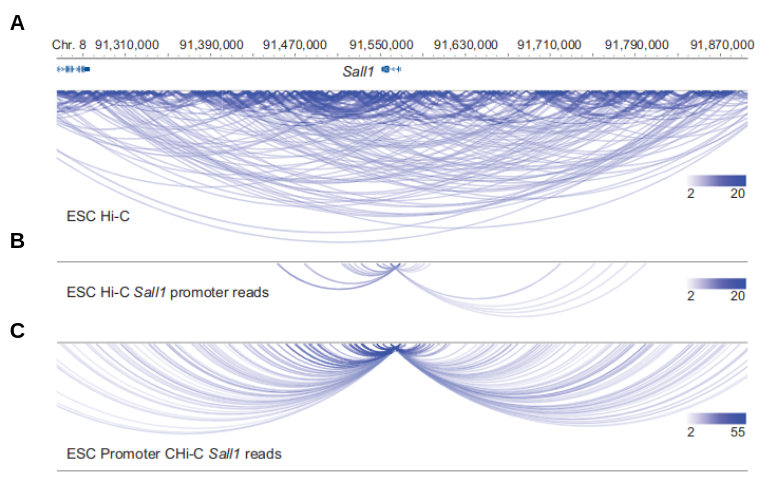
\includegraphics[width=0.8\textwidth, page=1] {figures/introduction/fig19.png}
 \caption[Comparaison des contacts de la chromatine mesurés par \acrshort{Hi-C} et par \acrshort{PCHi-C}.]{
 \textbf{Comparaison des contacts de la chromatine mesurés par \acrshort{Hi-C} et par \acrshort{PCHi-C}.}
 \textbf{A.} Interactions détectées en \acrshort{Hi-C} dans une région de 0.6Mb contenant le gène \textit{Sall1} dans les cellules souches humaines. L'intensité de la couleur d'une interaction indique le nombre de paires de lectures de séquençage entre deux séquences contactées. \textbf{B.} Même expérience de \acrshort{Hi-C}, mais seules les interactions qui mettent en contact le promoteur du gène \textit{Sall1} sont montrées. \textbf{C.} Interactions détectées en \acrshort{PCHi-C}qui contactent le promoteur de \textit{Sall1}. Le nombre de paires de lectures sur l'ensemble de l'échantillon a été ajusté pour être équivalent entre \acrshort{Hi-C} et \acrshort{PCHi-C}. Tirée de \citet{schoenfelder_pluripotent_2015}.\\
 }
 \label{fig:Fig19}
\end{figure}


\section{Le paysage \textit{cis}-régulateur}
\label{sec:paysage-cis-regul}

Afin de comprendre les déterminants de l'expression d'un gène il est alors important de pouvoir décrire l'ensemble de ses relations \gls{cis}-régulatrices. Les études qui se sont attachées à décrire ces relations ont alors fait émerger la notion de paysage \textit{cis}-régulateur de l'expression.

\subsection{Evolution de la définition du paysage \textit{cis}-régulateur}
\label{subsec:evol-def}

Ce terme de paysage a d’abord vu le jour à partir de l’observation de la structure hétérogène de la chromatine : les différences de compaction de l’ADN le long du génome ainsi que la variabilité des marques épigénétiques ont permis de définir un “paysage de chromatine” associé à l’activité des gènes \citep{grewal_heterochromatin_2003}. Un tel paysage ne permet pas à lui seul de décrire les relations régulatrices entre les gènes et les éléments \gls{cis}-régulateurs. Cependant il définit des grandes régions génomiques où la chromatine est dans un état qui permet ou pas l’expression des gènes. \\

Un autre type de paysage régulateur de l’expression des gènes a ensuite été défini à partir de la découverte de régions génomiques contenant plusieurs \glspl{amplificateur} régulant des gènes co-exprimés voisins \citep{spitz_global_2003}. Certains gènes agissent de manière coordonnée, par exemple pour former des complexes multi-protéines ou alors pour fonctionner dans les mêmes voies métaboliques. Ils peuvent être co-régulés par des éléments \gls{cis}-régulateurs communs et être regroupés dans une région génomique restreinte. C’est par exemple le cas des gènes \textit{HOX} qui sont responsables de nombreux processus développementaux, et qui sont regroupés dans certaines régions génomiques et peuvent être régulés par des \glspl{amplificateur} distaux communs \citep{spitz_global_2008}. D’après ces observations sur les gènes co-régulés, le paysage régulateur représenterait l’intervalle d’ADN à l’intérieur duquel l'ensemble des gènes est sous l’influence d’une même région régulatrice (Figure \ref{fig:Fig20}) \citep{spitz_global_2003}. Avec cette définition, la taille d’un paysage régulateur peut être variable selon le nombre d’éléments \gls{cis}-régulateurs y étant présents et selon les types cellulaires. \\

\begin{figure}[h]
 \centering
 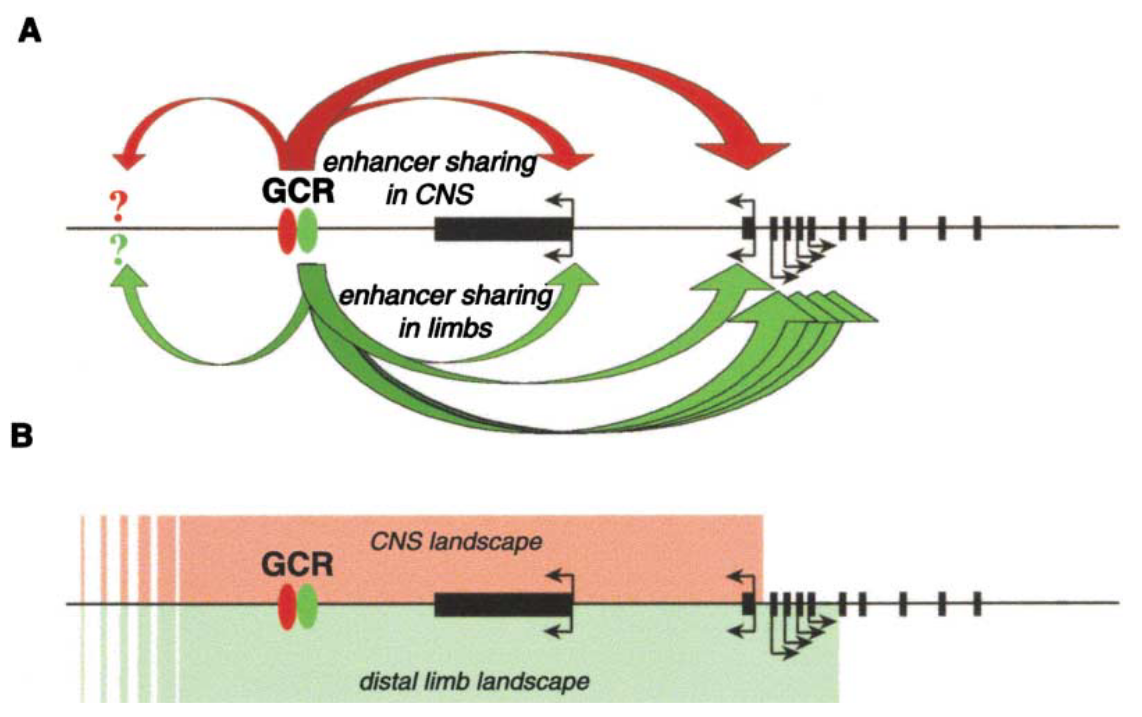
\includegraphics[width=0.8\textwidth, page=1] {figures/introduction/fig20.png}
 \caption[Première vision d'un paysage \gls{cis}-régulateur.]{
 \textbf{Première vision d'un paysage \gls{cis}-régulateur.}
 \textbf{A.} Une région riche en \glspl{amplificateur} (GCR pour global control region) peut contrôler l'expression de plusieurs gènes distants co-actifs. L'influence de cette région peut être variable selon les types cellulaires, en rouge co-activation des gènes dans le système nerveux central (CNS), en vert co-activation d'un plus grand nombre de gènes dans le développement des membres. \textbf{B.} Selon les types cellulaires, les frontières du paysages régulateurs pourraient donc être différentes. Tirée de \citet{spitz_global_2003}.\\
 }
 \label{fig:Fig20}
\end{figure}

De nombreux éléments \gls{cis}-régulateurs sont localisés tels des îlots dans les déserts de gènes autour des regroupements de gènes \textit{HOX} (Figure \ref{fig:Fig21}.A) \citep{montavon_regulatory_2011}. L’étude de l’organisation spatiale de la chromatine a révélé que certains de ces éléments \gls{cis}-régulateurs sont amenés de manière indépendante ou simultanée au voisinage du gène \textit{Hoxd13} par des boucles d’ADN \citep{montavon_regulatory_2011}. Ces interactions permettent une robustesse de l’expression de \textit{Hoxd13} tout en affinant de manière spécifique son activité dans plusieurs contextes distincts. Dans l'étude de Montavon et collaborateurs, les paysages régulateurs deviennent alors des ”archipels régulateurs” où les gènes peuvent être en interaction avec différents îlots  d’éléments \gls{cis}-régulateurs indépendants. \\

\begin{figure}[h]
 \centering
 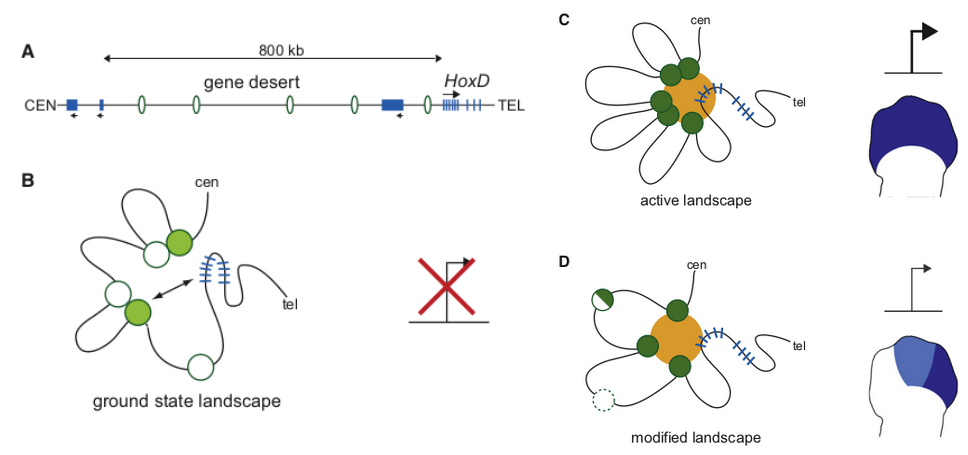
\includegraphics[width=1\textwidth, page=1] {figures/introduction/fig21.png}
 \caption[Notion d'archipel régulateur.]{
 \textbf{Notion d'archipel régulateur.}
 \textbf{A.} Segment génomique représentant un désert de gène dans une région de 800kb autour du promoteur de \textit{HoxD13}. Les rectangles bleus représentent des gènes et les cercles verts des îlots d'éléments \gls{cis}-régulateurs. \textbf{B.} Représentation de la conformation de la chromatine lorsque le gène \textit{HoxD13} n'est pas exprimé. Certains îlots possèdent des marques épigénétiques d'\glspl{amplificateur} actifs (rond vert plein) et peuvent contacter le promoteur du gène mais ne suffisent pas à initier sa transcription. \textbf{C.} \textit{HoxD13} est en contact avec l'ensemble des îlots actifs, il est exprimé de manière homogène dans le tissu. \textbf{D.} \textit{HoxD13} est en contact avec une partie des îlots et présente un patron d'activité différente. Tirée de \citet{montavon_regulatory_2011}. \\
 }
 \label{fig:Fig21}
\end{figure}

La définition de paysage \gls{cis}-régulateur évolue ensuite avec l’accumulation d’exemples de relations régulatrices à grande distance entre des promoteurs et des éléments \gls{cis}-régulateurs \citep{montavon_landscapes_2012}. Des cas comme celui de \acrshort{SHH} et \acrshort{ZRS} où la régulation s’effectue à très grande distance génomique, outre-passant plusieurs gènes, et n'activant aucun autre gène voisin, permettent d’en savoir plus sur les modes d’action des éléments \gls{cis}-régulateurs. C’est grâce au développement récent des techniques de capture de conformation de la chromatine (notamment les approches de types \acrshort{Hi-C}) que les paysages \gls{cis}-régulateurs peuvent aujourd’hui être mieux décrits et investigués à l’échelle du génome complet. \\

Au cours de cette thèse, je définirai donc le paysage \gls{cis}-régulateur d’un gène comme l’ensemble des éléments \gls{cis}-régulateurs qui peuvent avoir un impact sur le niveau ou l’étendue de son expression. Cette définition évoque un paysage complexe à déterminer : les sous-ensembles d’éléments \gls{cis}-régulateurs d’un gène peuvent être différents selon l’étape de division cellulaire, le stade de développement, le type cellulaire, les facteurs environnementaux, etc.. Il apparaît ambitieux d’avoir une mesure ou une connaissance exhaustive du paysage \gls{cis}-régulateur d’un gène. Cependant la multiplication des expériences, notamment par des mesures des contacts de chromatine, dans un grand nombre de contextes permet d’en obtenir un aperçu.

\subsection{Complexité du paysage \textit{cis}-régulateur et patron d’expression des gènes}
\label{subsec:complexite}

Les paysages \gls{cis}-régulateurs de l’expression des gènes peuvent mettre en relation de nombreuses séquences fonctionnelles. Chaque gène peut en effet être associé à plusieurs éléments \gls{cis}-régulateurs et inversement chaque élément peut contrôler plusieurs gènes. Ces associations peuvent se faire de manière simultanée par des boucles de la chromatine qui co-localisent plusieurs éléments. Par exemple, il a été montré qu’un \gls{amplificateur} peut réguler simultanément deux gènes distants l’un de l’autre sur le génome linéaire \citep{fukaya_enhancer_2016}. Plusieurs \glspl{amplificateur} peuvent être nécessaires pour activer la transcription d’un gène, en recrutant différents facteurs de régulation en \gls{trans} par exemple. Les \glspl{amplificateur} peuvent également avoir des fonctions partiellement ou totalement redondantes sur l’expression des gènes cibles. Cette redondance pourrait assurer une robustesse de l’expression des gènes cibles \citep{berthelot_complexity_2018}. En augmentant le nombre d’\glspl{amplificateur}, la probabilité de rencontre entre un gène et un \gls{amplificateur} est en effet augmentée, ce qui augmente les chances que la transcription soit initiée. De plus, il a été montré que le nombre d’\glspl{amplificateur} avec lequel un gène interagit est corrélé positivement avec son niveau d’expression \citep{schoenfelder_pluripotent_2015, mifsud_mapping_2015, javierre_lineage-specific_2016, berthelot_complexity_2018}. Ceci suggère un effet additif des \glspl{amplificateur} qui permettraient une augmentation de la fréquence des cycles d’activité de la transcription du gène \citep{bartman_enhancer_2016}. Certains \glspl{amplificateur} ont cependant des fonctions non redondantes et sont obligatoires pour assurer la transcription du gène dans un contexte donné. \\

\begin{figure}[hbt!]
 \centering
 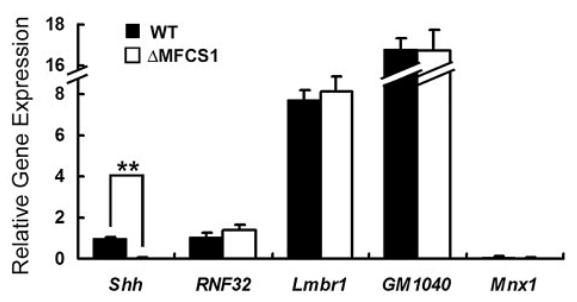
\includegraphics[width=0.7\textwidth, page=1] {figures/introduction/fig22.png}
 \caption[Impact de la délétion de \acrshort{ZRS} sur l'expression de ces quatre gènes voisins et du gène \acrshort{SHH} distal.]{
 \textbf{Impact de la délétion de \acrshort{ZRS} sur l'expression de ces quatre gènes voisins et du gène \acrshort{SHH} distal.}
 Expression relative des gènes dans le bourgeon des membres inférieurs d'embryon de souris avec un génotype sauvage (noir) ou étant homozygotes pour la délétion de \acrshort{ZRS} (précédemment nommé MFCS1) (blanc). Les niveaux d'expression des gènes sont normalisés par le niveau d'expression du gène de ménage de la Beta-actine. Le niveau d'expression de \acrshort{SHH} dans l'embryon sauvage est pris comme référence. Les barres d'erreur représentent les écarts types obtenus à partir des expériences réalisées sur trois réplicats. Les doubles astérisques indiquent des différences significatives, évaluées par le test t de Welch (p $<$ 0,01).Tirée de \citet{amano_chromosomal_2009}.\\
 }
 \label{fig:Fig22}
\end{figure}

Un élément \gls{cis}-régulateur peut réguler l’expression de plusieurs gènes en même temps et/ou dans des types cellulaires différents, et ainsi avoir de nombreuses fonctions. Les \glspl{amplificateur} seraient majoritairement spécifiques d’un tissu, indépendamment des gènes qu’ils régulent \citep{singh_enhancer_2021}. Certains \glspl{amplificateur} sont en effet très spécifiques comme c’est le cas de \acrshort{ZRS} qui semble réguler uniquement \acrshort{SHH} et uniquement dans le développement des membres. La délétion de celui-ci dans le génome de la souris réduit significativement l’expression de \acrshort{SHH} sans affecter l'expression des quatre gènes avoisinant \acrshort{ZRS} (Figure \ref{fig:Fig22}) \citep{amano_chromosomal_2009}. Il est cependant difficile d’estimer précisément l’ensemble des gènes cibles d’un \gls{amplificateur}. Bien que cela n'ait pas été testé, \acrshort{ZRS} pourrait par exemple affecter d’autres gènes plus distaux ou des gènes dans des contextes cellulaires différents. Le gène \acrshort{SHH} est cependant très \gls{pleiotrope} et assure différentes fonctions dans plusieurs types cellulaires. L’expression de \acrshort{SHH} est régulée par plusieurs \glspl{amplificateur} spécifiques de différents tissus et situés dans une large région s’étendant à plus de 1Mb autour du gène \citep{epstein_regionalization_1999, lettice_long-range_2003}. \\

C’est donc l’interaction modulable des éléments \gls{cis}-régulateurs avec un gène cible, conjointement avec l’état de la chromatine et la présence de facteurs agissant en \gls{trans}, qui permet d’établir son patron d’expression pour chaque type cellulaire (Figure \ref{fig:Fig23}). Le paysage \gls{cis}-régulateur permet d’affiner précisément le patron d’expression d’un gène dans chaque type cellulaire. De par la possible complexité du paysage \gls{cis}-régulateur d'un gène, une importante modularité des éléments \gls{cis}-régulateurs est possible. C'est-à-dire que différentes configurations à partir d'un même ensemble d'élements \gls{cis}-régulateurs pourrait permettre aux gènes d’être actifs dans un plus grand nombre de types cellulaires et d’être impliqués dans un plus grand nombre de fonctions métaboliques. Finalement, la redondance d’un tel réseau de régulation peut permettre une plus grande tolérance aux mutations et serait alors en mesure de participer à une forte plasticité et évolution de l’expression des gènes.

\begin{figure}[h]
 \centering
 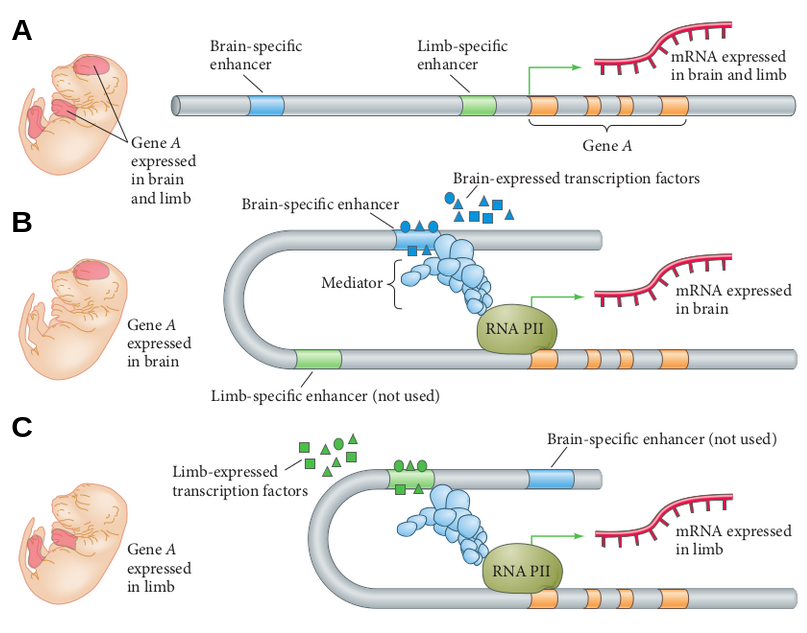
\includegraphics[width=0.9\textwidth, page=1] {figures/introduction/fig23.png}
 \caption[Modularité du paysage \gls{cis}-régulateur.]{
 \textbf{Modularité du paysage \gls{cis}-régulateur.}
 \textbf{A.} Schéma modèle d'un gène A, composé de 4 exons (orange), exprimé dans le cerveau et les membres au cours du développement. Son paysage \gls{cis}-régulateur est composé d'au moins deux \glspl{amplificateur} : l'un spécifique du cerveau (bleu) un autre des membres (vert). 
 \textbf{B.} Dans le cerveau, des facteurs de transcription se fixent sur l'\gls{amplificateur} spécifique. Ceci permet de recruter diverses protéines qui vont changer la structure de la chromatine et recruter l'\acrshort{ARN} polymérase II pour transcrire le gène A. L'\gls{amplificateur} spécifique des membres n'est pas utilisé, par exemple à cause de modification épigénétique particulière ou d'absence d'éléments \gls{trans}-régulateurs spécifiques de sa séquence.
 \textbf{C.} Scénario similaire dans les membres, où le gène A est transcrit grâce à l'\gls{amplificateur} spécifique de ce tissu. Le gène n'est pas activé dans d'autres \glspl{condition} où les facteurs de transcription ne peuvent se lier à l'un de ces deux \glspl{amplificateur}.
 Tiré de \citet{gilbert_developmental_2017}.
 }
 \label{fig:Fig23}
\end{figure}

